      \chapter{Beyond the Talking Heads Experiment}
\label{c:postscriptum}
%\newcounter{foot}
\setcounter{foot}{1}

The Talking Heads experiments were obviously not an end point, but only the beginning. They confirmed the results that 
had been obtained with earlier theoretical models and computer simulations but did not push these models 
towards greater complexity. But subsequent work did expand the envelope of our understanding and modeling way  
beyond these boundaries, thanks to the work of many researchers who have since joined the research program. 
The expansion has happened along several dimensions: increased sophistication of the robots, a deeper theoretical 
understanding of semiotic dynamics, growth in the complexity of semantics and grammar, and new breakthroughs by 
studying the emergence and evolution of language strategies. An exhaustive survey of these exciting profound developments 
is beyond the scope of the present book. Instead, I will highlight here only some of the key language game experiments that 
used real physical robots and were direct variations or further extensions of the environments, game scripts
and strategies used in the Talking Heads experiment. This chapter focus on experiments 
in the period  before 2005, particularly work with the AIBO robots and the first attempts towards the emergence 
of grammar.\footnote{An overview of these experiments is also given in \cite{Steels:2005}.}
The next chapters focus on experiments after 2005. 

\section{Experiments with the AIBO robots} 

From 1996, even before the first Talking Heads experiment was started, experiments were already conducted in our 
laboratory, primarily by Paul Vogt, exploring language games on the cybernetic mobile robots that we were able to build ourselves
at the time. These robots were constructed from Lego bricks and 
used a basic processing board for linking directly simple sensors (touch sensors, infrared sensors) and actuators (left and right motors)
using an adaptive dynamical system (see \figref{f:plate3}). They were however too unreliable for long-term repeatable 
experimentation and the sensori-motor experiences were too restricted to hope for the development of interesting languages. The use 
of pan-tilt cameras, as in the Talking Heads experiment, was an attempt to 
have an experimental set-up at relatively low cost that was reliable and
used vision as the source of information about the world. Of course this came
at the price of less mobility and no true physical interaction with the real world. Nevertheless, many further fruitful experiments were 
done using the same set-up, particularly to explore in much greater depth the domain of color lexicons
\footnote{Colour became a focal point of research because there is an extensive literature in cognitive science that has 
been gathering empirical data about color and its evolution and because it is relatively straightforward to do 
colour naming games. One of the main papers on our colour naming research is: 
\cite{Steels:2005}} and multi-word naming games\footnote{Multi-word games were the focus of the ph.D research by 
Joris Van Looveren, with a thesis defended in 2004.}
A Talking Heads simulator was also built by Paul Vogt\cite{Vogt:2003} in 
order to speed up such experiments and prepare the way for more advances with real robots.

\subsection{AIBO's First Words}

Meanwhile significant developments started to happen in the world of robotics that pushed the state of 
the art in fully-embodied mobile robots forward.  
Around the year 2000, a new generation of robots was becoming available, built 
by industrial companies which mastered the technology to manufacture very robust machines, and these robots could therefore
be used continuously without constant breakdown. Because of experience and contacts in the field of
robotics, our team was able to move language game experiments to a new level of sophistication. The first 
platform we could use was the Sony AIBO robot. \is{AIBO}

The AIBO is a fully autonomous 4-legged mobile robot, inspired by a small dog. It is fully autonomous with more than 
a thousand behaviors coordinated through a complex behavior-based motivational 
system.\footnote{This robot was entirely based on a series of design principles that I had pioneered together with Rodney 
Brooks in the mid-nineties under the label 'behavior-based AI'. See: \cite{Steels:1995}, \cite{Steels:1994}.}
The robot was pioneered by
Toshi Doi and designed by Masahiro Fujita and his team at the Sony Corporation in Tokyo at the end of 
the nineties.\cite{Fujita:1998}
In all 150,000 AIBO's were sold to customers. The AIBO featured 4-legged locomotion, 
a camera for visual input, two microphones, a wide range of body sensors, on-board batteries and the necessary 
computing power. This robot was the most complex reliable robot available in the early 2000's. 
The AIBO was also the first robot that was explicitly designed for 
human interaction so that basic useful components (for example for face recognition) were available. Language game research
could therefore focus entirely on the linguistic and conceptual aspects of the semiotic cycle, even though 
we still had to program the physical interaction patterns and behaviors necessary for language games. 

Language Game experiments started on the AIBO when the Talking Heads experiment 
was still going on, namely in 2000. Fr\'{e}d\'{e}ric Kaplan was the main developer.\footnote{A paper summarising 
the AIBO experiment was published as \cite{Steels:2001}. Kaplan wrote his ph.D thesis on the subject 
which is published (in French) as \cite{Kaplan:2001}.}

These experiments extended the Talking Heads experiment in several directions: 
\begin{enumerate}
\item {\itshape Vision.} The pan-tilt cameras and the flat white board with geometric figures ensured that the vision system 
of the Talking Heads was relatively reliable, although light conditions and camera misalignment
could occasionally 
cause havoc. The AIBO experiments now used 3d objects in the real world that were seen from many different 
angles and in different light conditions (see \figref{f:look-ball}, right). This obviously pushed up the 
difficulty of visual perception enormously and it also made it much more difficult to acquire stable categories 
for reliably recognising the objects in the environment. 
\item {\itshape Speech.} The interaction with the robot used spoken language, which implied that the robot needed 
speech synthesis and a speech recognition system that could acquire new words. These components were available on the 
robot and could therefore be easily integrated. 
\item {\itshape Flexible scripts.} The Talking Heads experiments used a single very streamlined interaction scenario whereby
the robots played a Guessing Game with a clear turn-taking script. The AIBO experiments targeted different 
kinds of interactions with humans and therefore the robot needed not only a way to represent and execute these 
different scripts but also a much more flexible way to move from one step to another within a script and to move 
between scripts. Moreover the scripts had to be integrated intimately with the physical behaviors that were 
steering the robot itself, which could in many cases not be overridden or directly controlled. 
\end{enumerate}


\begin{figure}[htbp]
  \centerline{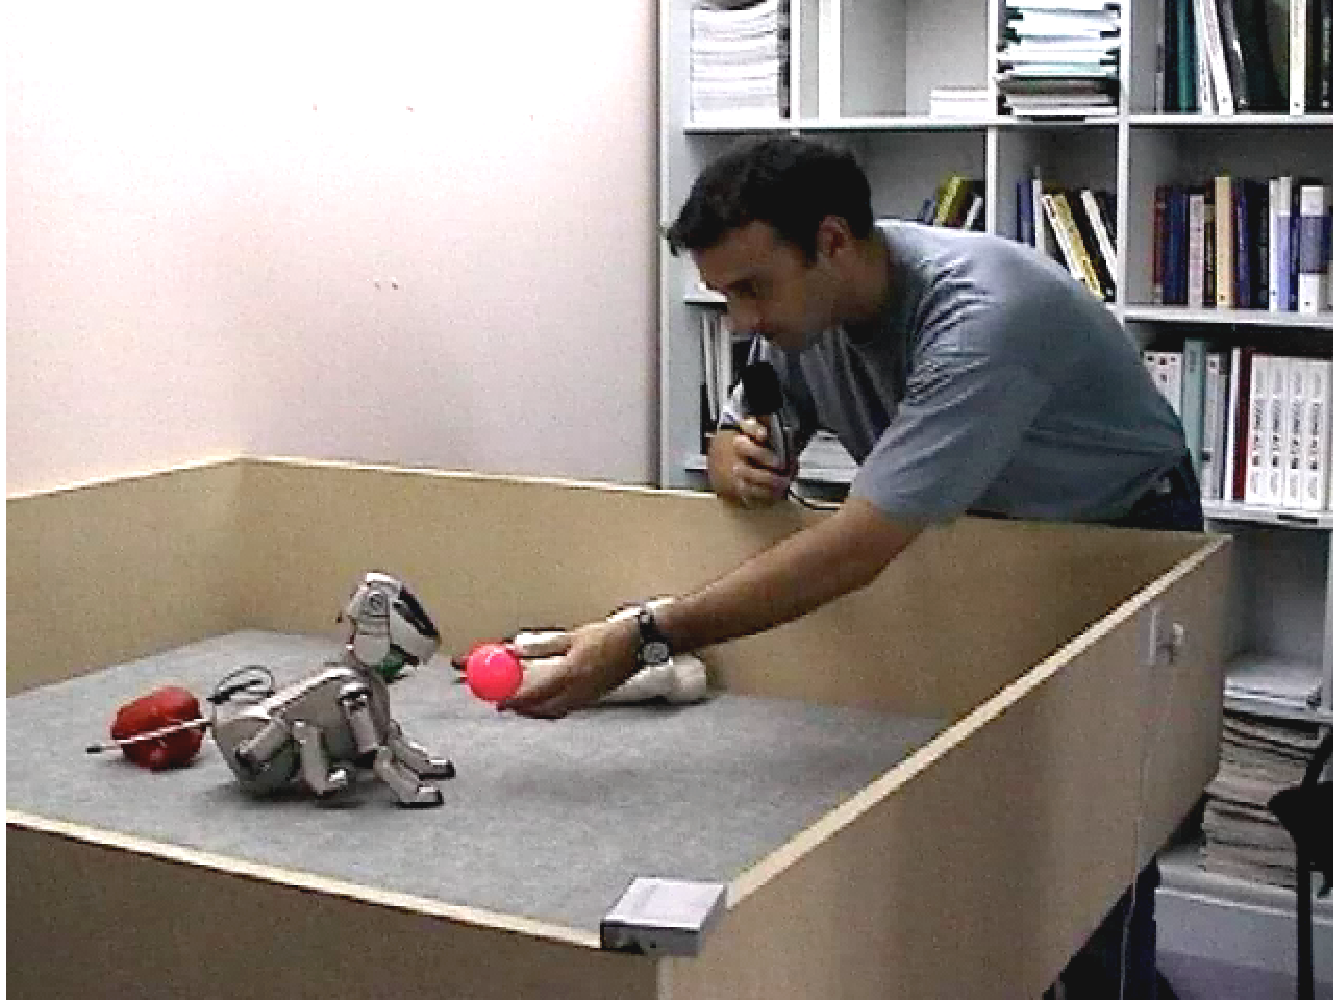
\includegraphics[width=.50\textwidth]{chap10/figs/look-ball}
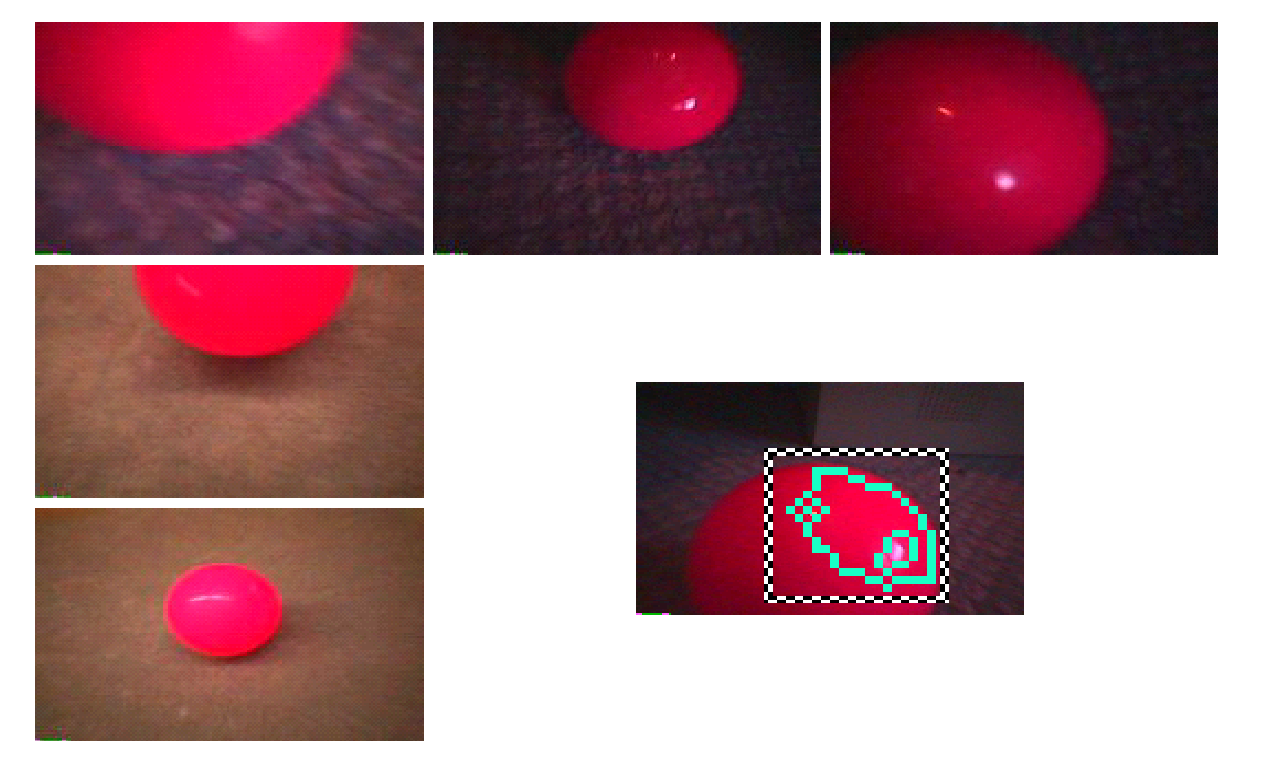
\includegraphics[width=.45\textwidth]{chap10/figs/views-ball}}
\caption{\label{f:look-ball} 
Left: Fr\'{e}d\'{e}ric Kaplan interacts with the AIBO robot in an experiment for the social learning of lexicons.
Right: View of the ball through the eye of the robot. As the same object is now seen from many different viewpoints it 
becomes much more challenging to consistently recognize it.}
\end{figure}
The first AIBO experiments did not involve a population of agents but rather a single agent that was interacting directly with a human
experimenter. The agent had to learn the lexicon of the human through social 
interaction within the context of situated language games. The 2001
paper ''AIBO's first words'' by Steels and Kaplan described experiments in which an AIBO robot 
learned words about objects in the environment, such as ``ball'' or ``smiley", as well as words for actions, such as 
``sit down'' or ``stand up". 

A typical example of a game is the DO game, used to learn the names of behaviors.\is{DO game} 
The robot is programmed with a repertoire of behaviors, such as 
walk, sit down, stand up, look left/right/up/down, push ball, etc. When the human utters a word, the hearing robot 
looks up the word in its own memory and performs that behavior. If it does not know the word, it 
performs one of the behaviors for which it does not have a word yet. 
If this behavior is the wrong one, the robot receives feedback and correction, 
thus learning (i) that the behavior is not associated with the word and (ii) what the right word is for the behavior 
just performed. When the right behavior was chosen, the association between this behavior 
and the word can be stored if the association was not yet in memory, or reinforced if it was using the 
lateral inhibition learning strategy. 
Games therefore always come with two variant scripts. There is one with a successful interaction, which then 
leads to a reinforcement of the existing lexicon, and one with a non-successful interaction, where the 
robot gets corrected and learns a new word. Here are the two variants for the DO Game: 
\begin{center}
\begin{tabular}{ l  l }
\lsptoprule
{\itshape Reinforcement script}&{\itshape Correction script} \\ \midrule
Human: Listen, Walk. & H: Listen, Walk.  \\ 
R: Walk? & R: Walk? \\
 {\itshape (walks)} & {\itshape (sits)} \\
H: Yes & H: No, this is ''sit". \\
& R: Sit ? \\ 
& H: Yes. \\ 
\lspbottomrule
\end{tabular}
\end{center}
The scripts of the agents are represented internally using probabilistic finite state machines with 
temporal annotations. This computational formalism (pioneered by Rodney Brooks) was also used to program the 
physical behavior of the robots (\figref{fig:fsm}).\footnote{
This architecture was first described in \cite{Brooks:1986} 
For the experiments I implemented a LISP-based Behavior Language that ran also on the AIBO.}

Each state in a behavior network \is{behavior network}
represents a decision point. A transition is an event happening in the real world or a condition in 
the internal memory of the agent. Occasionally there is more than one possible continuation from a state 
and a transition is then decided purely based on a probabilistic basis.  
When waiting for events in the environment, the transitions have a timer, so that the robot can recover when an 
expected event is not occurring. In the subsumption architecture networks are stacked and
one network may overtake another one. For example, an obstacle avoidance behavior will become active when 
touch, vision or infrared sensing has 
detected an object, whatever other network is governing at that time the robot behavior. 

\begin{figure}[htbp]
  \centerline{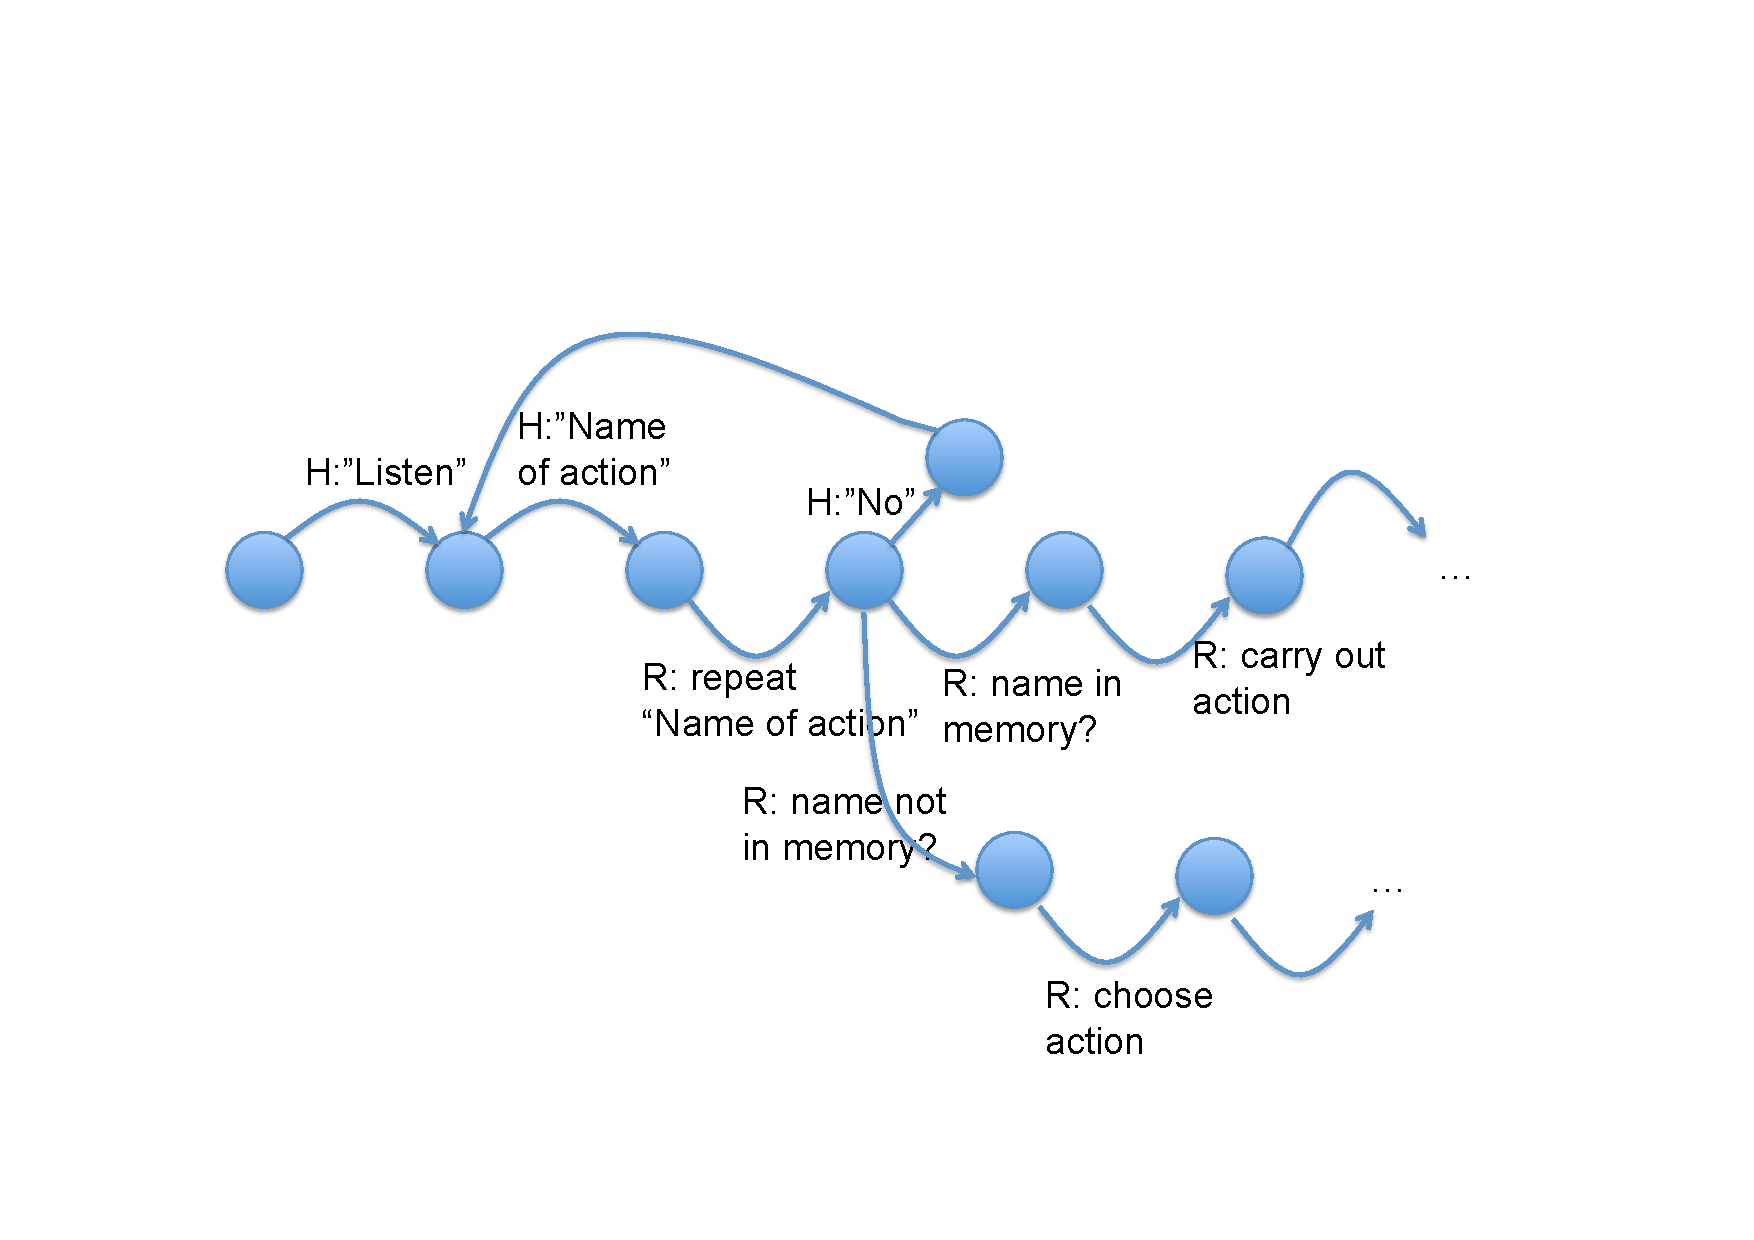
\includegraphics[width=.70\textwidth]{chap10/figs/fsm}}
\caption{\label{fig:fsm} 
The behavior on the AIBO, including the language game scripts, are programmed using probabilistic finite state 
machines that bring the robot from one internal state to another one depending on internal or external conditions.}
\end{figure}

The main conclusion of these experiments was that the state of the art in robotics and language
game research was sufficiently advanced at that time (i.e. in 
2001) to implement these more complex games. Moreover several experiments were done to compare
different learning methods and interaction patterns, comparing social, situated learning with 
observational learning. In social situated learning, \is{social situated learning}
the learner maximally uses information from the context, the 
interaction, and the existing state of his language system, to make the best possible guess about the meaning of 
unknown utterances. He gets help from the speaker which is acting as a tutor and gives useful feedback to constrain 
the uncertainty as much as possible. An utterance is seens as purposeful and the hearer assumes that the speaker conceptualises
and expresses what is relevant to achieve communicative success. In observational learning, the learner is 
passively observing interactions of others and stores them as data. When there is a sufficiently big 
corpus he can employ cross-situational learning to grasp the meaning of each word by scanning 
through the data to find the commonalities between 
situations using the same word. This approach works also to some extend but experiments showed that it was much slower and 
not so easily made incremental.\cite{DeBeule:2006}

The AIBO experiments were the first robotic experiments demonstrating social, situated learning in action. 
They were highly relevant for discovering the subtle interaction patterns that would work and 
could be realistically implemented in human-robot scenarios. The goal of these experiments was 
not to address the question of the origins of a 
new language in a population of agents. However, another experiment, still with the AIBO robots,  
did substantially advance the state of the art: the Perspective Reversal Experiment carried out by Martin Loetzsch 
and Luc Steels in 2004-2005.\footnote{
Very little was published about this experiment, partly because reviewers had the greatest difficulty to grasp 
its underlying rationale or understand the technical details. The main paper is \cite{Steels:2008spatial}. 
Subsequent work by Michael Spranger significantly scaled up the experiment, as discussed in the next chapter.}

\subsection{The Perspective Reversal Experiment}

The Perspective Reversal Experiment \is{Perspective Reversal} focused on the question how a spatial language could emerge that employed
perspective reversal. It was the first experiment to systematically compare different language strategies, thus 
introducing for the first time the {\itshape comparative method} \is{comparative method} 
that would inform all later language game experiments. 

A {\itshape language strategy} \is{language strategy} 
prescribes how some aspect of meaning needs to be conceptualised, expressed, and acquired. 
The Talking Heads experiment used a single strategy: find a discriminating category for the topic and employ a word 
for that category. But languages use a variety of strategies all intermixed. 
For example, speakers might have a strategy for expressing argument structure using cases (as in Latin or German) or 
a strategy for expressing tense and aspect using morphological markers on the verb (as in Spanish). Each strategy gives 
rise to a particular feature of a language and in order to demonstrate why languages exhibit this feature it is therefore
possible to compare a language with the feature to one without the feature by doing an experiment where
agents are endowed with a strategy that generates this feature and another one where they employ a different strategy
that does not. The performance of the resulting system, for example, its average communicative success, the time to reach 
linguistic convergence, the amount of cognitive effort involved, can be measured and thus the adaptive value of one 
strategy (and hence one feature of language) can be compared with another. 

The comparative method fits within the larger framework of selectionist theories  
of language origins, which argue that language users are able to configure strategies by recruiting and configuring 
cognitive mechanisms (such as sequence detection, categorisation, perspective reversal, etc.) and that those 
strategies that make a positive contribution to the language are retained.\footnote{
More on the recruitment theory of language origins in: \cite{Steels:2007recruitment}. 
And on the selectionist framework in general in \cite{Steels:2012}.}
The strategies being compared have to form a chain where one strategy is a slight variation on the previous one, typically 
an additional component is begin recruited and linked into the strategy, so that we can begin to imagine an 
evolutionary trajectory in which strategies progressively complexify (see section 11.1.2)

The Perspective Reversal Experiment applied this methodology to explain a remarkable universal feature 
of human languages, namely, 
that speakers may use a different perspective on the scene than their own when 
conceptualizing what to say, and that they may explicitly mark perspective switching, using lexical or grammatical means. Suppose
a speaker is facing a hearer, then it indeed makes a big difference whether she says 
\emph{the door to your left}  or \emph{the door to my left}. If the speaker says
\emph{the door to my left} she expects the hearer to perform an egocentric
perspective transformation and see the situation from her own point of view. Perspective switching is here signalled by 
explicitly expressing which perspective is used: {\itshape your} left versus {\itshape my} left. 
The German prepositions \emph{herein} and \emph{hinein}, both meaning ``inside'' are another example of perspective marking. They
distinguish whether the direction of movement is 
towards the speaker \emph{herein} or away from the speaker \emph{hinein}, analogous to English \emph{come} (to where I am) 
versus \emph{go} (to another location). Although there are obvious differences in how languages express
perspective, there can be no doubt that perspective marking is pervasive across 
languages and language families, and that speakers make abundant use of it. 

\begin{figure}[htbp]
  \centerline{\includegraphics[width=.65\textwidth]{chap10/figs/tokyo-persp}}
\caption{\label{fig:tokyo-persp} 
Luc Steels demonstrates live the Perspective Reversal Experiment in Tokyo, April 2005. AIBO robots track 
the movement of a ball and 
the robot acting as speaker describes to the hearer an observed movement, possibly taking into account the 
perspective of the hearer. For example, the speaker might say ``the ball rolls from my left to your right".}
\end{figure}

The Perspective Reversal Experiment worked as follows. A population of AIBO robots roam around
freely in an unconstrained in-door environment. As soon as one sees the
ball, it comes to a stop and searches for another robot nearby, which also
looks for the ball and stops when it sees it. Then the human
experimenter pushes the ball with a stick so that it rolls a short
distance (see \figref{fig:tokyo-persp}). The two robots next play a description game. One robot (acting as the `speaker') 
describes the ball-moving event to the other robot (the `hearer'), going through the same semiotic cycle as the Talking 
Heads agents. The game is a success if the meaning conveyed by the speaker is compatible with the hearer's 
own perception of the scene. 

The robots start without any prior lexicon or ontology and have to come up with their own 
purely based on the feedback in the game and without any human intervention. 
They have been programmed to achieve autonomous locomotion and vision-based obstacle avoidance,
and maintain a real-time analog model of their immediate surroundings based on visual input. Using
this vision-based world model, the robots are able to detect and track
other robots as well as orange balls using standard image processing
algorithms (see \figref{fig:persp-rev-perception}). Furthermore, the
robots have been endowed with mechanisms to segment the flow of data
into distinct events and they have a short term memory in which they
can store a number of past events.

\begin{figure}[htbp]
  \centerline{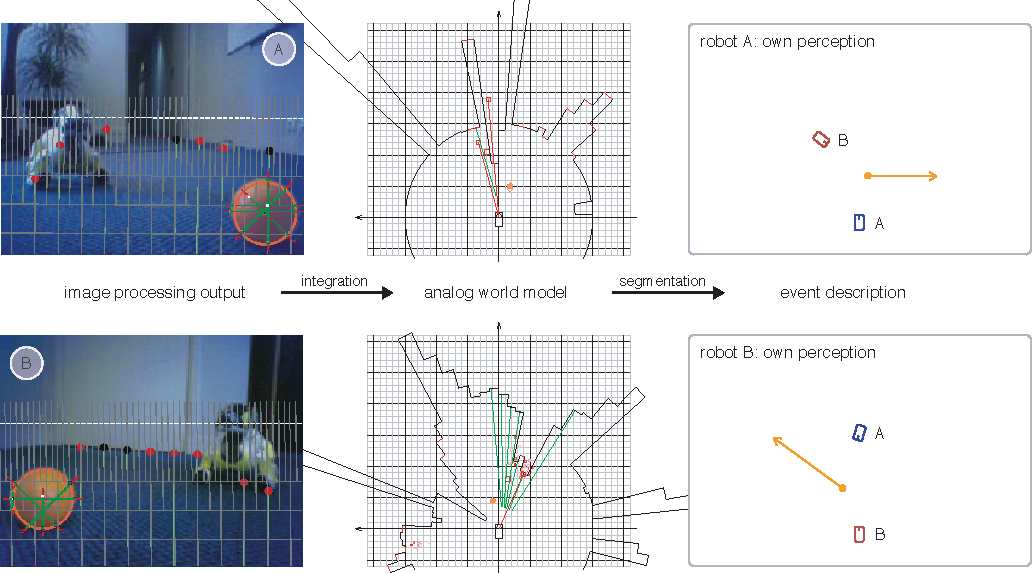
\includegraphics[width=.90\textwidth]{chap10/figs/persp-rev-perception}}
\caption{\label{fig:persp-rev-perception} 
Chain from visual image (left) to an analog world model (middle) and a discrete event description
that is the topic of the language game (right). 
The top row shows this chain for robot A and the bottom row the chain for robot B, both looking at the same ball.}
\end{figure}

Within this experimental setting three different strategies were tried in a long-term experiment where
a new strategy was injected at certain stages and performance monitored: 
\begin{itemize}
\item In stage I, agents use 
the Discrimination Game strategy and the Naming Game strategy discussed in chapters 4 and 5. A 
lexicon is emerging and there are some successful games (those for which the speaker and the hearer see the situation from 
the same perspective). But the lexicon keeps expanding and success is very limited as games where robots have a different 
perspective on the rolling ball all fail. 
\item In stage II, agents have an extended 
strategy where agents can geometrically transform a model of the scene, based on their own perspective, into a model of the scene 
as seen from the perspective of the hearer. They can then conceptualise the scene from that perspective. 
Communicative success significantly increases and the 
lexicon starts to decrease. However there is ambiguity because the hearer cannot know whether
the speaker has conceptualized the 
scene from his own viewpoint or performed a perspective reversal, leading to a large number of failed communications 
(more than 50 \%). 
\item In stage III, a more elaborate stratergy is used. The speaker now expresses whether he has performed perspective 
reversal (as in ``{\itshape to your} left'' vs. simply ``left''). Only with this strategy are agents able to reach high 
communicative success with a stable inventory. 
\end{itemize}


\begin{figure}[t]
\centerline{
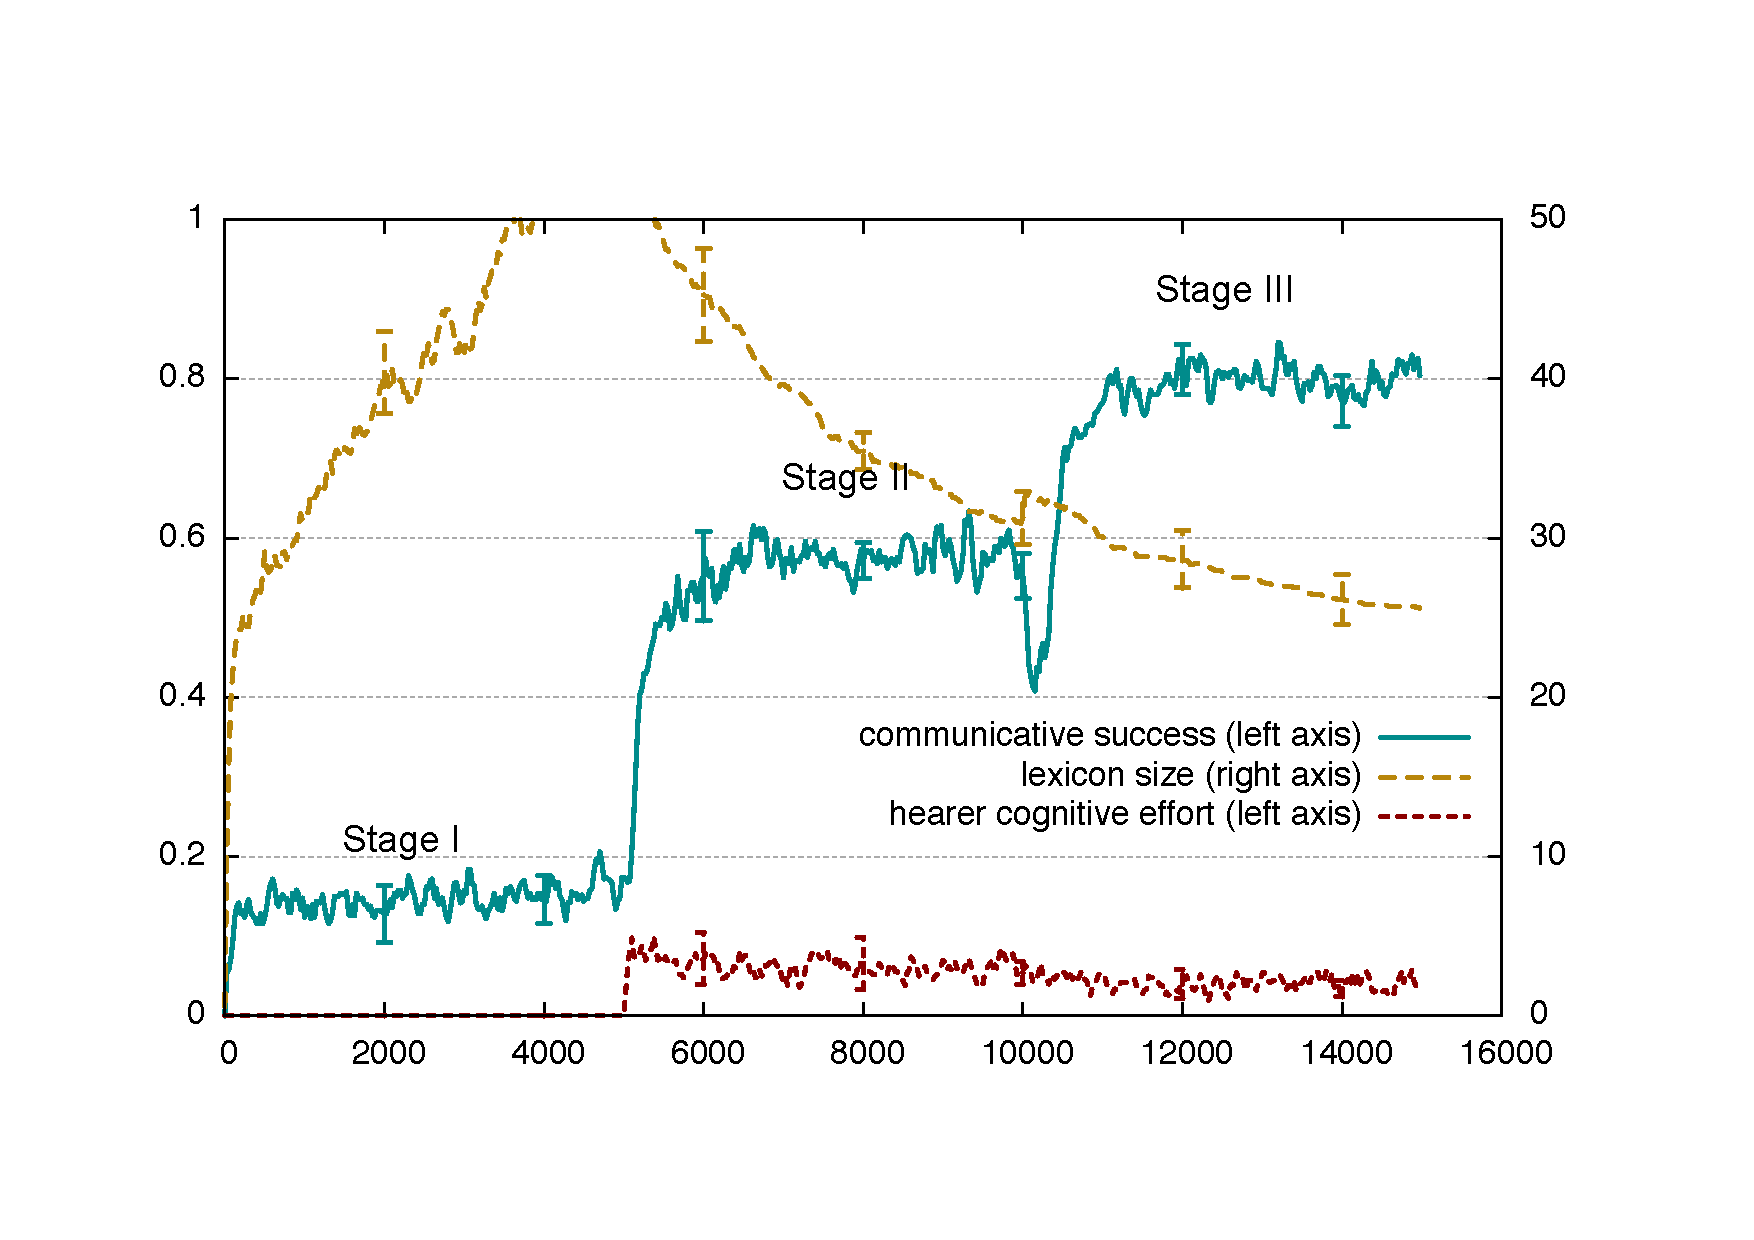
\includegraphics[width=0.75\textwidth]{chap10/figs/stages}}
\caption{\label{fig:stages} 
Three strategies are compared. In Stage I (left) agents categorise the event from their 
own perspective. In Stage II (middle) they conceptualise the scene from the viewpoint of the other agent as well. In Stage III (right) 
they express that they performed a perspective reversal. Only the third strategy leads to successful performance.} 
\end{figure}

The Perspective Reversal experiment was significant in many ways. Not only did it use for the first time mobile robots in a 
sophisticated open real world set-up, but it also pioneered the use of perspective reversal that was the basis of later 
experiments in spatial language games with the QRIO robot by Michael Spranger and it was the first convincing example of 
the comparative method that now underlies all advanced language game research. What this experiment did not address
was how agents could come up with new strategies themselves and how more adapted strategies could propagate and become 
shared in the population. 

\section{Scaling up to Grammar}

We now look at other dimensions in which language game research moved beyond the original 
Talking Heads experiment.\is{grammar emergence} 
The original experiments focused exclusively
on the question how a vocabulary of grounded concepts could arise in a population 
of agents. Agents could already use multiple word utterances but without any notion of grammar. 
The obvious next question was how all this could scale-up towards grammar. This is of course an extremely difficult
challenge that required significant advances both for the representation of the linguistic inventory 
available to the agents and how meaning is expressed and interpreted. As common in 
scientific and engineering research, we moved step by step, systematically adding more complexity but 
testing out each step before moving to the next one, and this progressive complexification is still on the way today.

\subsection{Early Syntax Experiments}

The earliest attempts to investigate the emergence of syntax date back to 1997, in other words even before 
the first Talking Heads experiment started. The first report 
appeared as a paper in the Artificial Intelligence journal in 1998.\cite{Steels:1998}. 
It was described by the journal editors (Dan Bobrow and 
Mike Bray) as ''obviously in an early stage, but very provocative and suggestive.'' The paper was based on my keynote 
lecture at IJCAI 1997 in Nagoya and used a precursor of the pan-tilt cameras built by Tony Belpaeme. 
(see \figref{f:plate7}). 

The paper describes the grammar formalism as follows:

"The grammar is seen as a natural continuation of the lexicon, in the sense that it consists also of associations between forms and meanings. Use and success are monitored for each association so that the same type of self-organized coherence arises in the group, as seen in the lexicon. The form is now a more complex structure, defined as a syntactic schema. The meaning is a semantic schema. The schemas
circumscribe a feature-set in terms of a set of slots, restrictions	
on the fillers of each slot, and constraints	on the combination	
of the fillers to form the total covered by the schema. 

Syntactic schemas describe word groups. They have an associated category which corresponds in linguistic terms to grouping categories like noun-group, verb-group, sentence. The slots in syntactic schemas correspond to syntactic functions (also called grammatical relations) such as subject, object, modifier, complement. They name the roles that certain words or word groups play in the group. The categories used to restrict possible slot-fillers correspond in linguistic terms to syntactic categories like noun, verb, adjective, etc. An example of a syntactic schema is the following:
\begin{verbatim}
Schema-541 
  SLOTS: (syn-slot-51 syn-slot-50) 
  DESCRIPTION-SET: 
      ([syn-slot-50 syn-cat-751] 
       [syn-slot-51 syn-cat-761])
  CONSTRAINTS:	((PRECEEDS (>> syn-slot-50) (>> syn-slot-51)))
  CATEGORY: syn-cat-77 
  USE: 10 
  SUCCESS: 3
\end{verbatim}
Of course, instead of noun, noun-group, subject, etc. computer-generated symbols are used such 
as syn-cat-77, syn-slot-50, etc. The constraints on the schema are represented in terms of
a constraint system. Each constraint
has a dual procedural function: to enforce the constraint when re-enacting the situation
described by a schema or to test the constraint when determining whether a schema fits with a situation. In the present
case only a precedence relation is recorded as a constraint. Agreement, intonation, or morphological
endings, are some other possible constraints on syntactic schemas.

The categories restricting slot-fillers are either themselves defined in terms of schemas
(for example, syn-cat-77 could be the restriction on a slot-filler in another schema), or they
are defined as rules that are applied in a forward-chaining fashion during matching. Two
examples of rules related to the above schema are:
\begin{verbatim}
  rule 101: ([WORD (W U)]) => ([MEMBER syn-cat-761])
  rule 99: ([WORD (W O)]) => ([MEMBER Syn-Cat-751])
\end{verbatim}
Semantic schemas describe the language-specific semantic structures underlying the
meanings of complete word groups. The closest linguistic correspondent to a semantic
schema is the notion of a case-frame. The constraints indicate how the total meaning
is constructed/decomposed into the meaning of the parts. During interpretation such
constraints therefore perform the same role as Montague style semantic interpretation
functions. The slots correspond to cases such as agent, patient, time, distance, or arguments
of semantic functions. The categories used to constrain what can fill a slot correspond
in linguistic terms to selection restrictions like animate, human, edible, future, etc. The
schema has also an associated category for the whole so that hierarchical combination is
possible. An example of a semantic schema is:
\begin{verbatim}
Schema-542
  SLOTS: (sem-slot-51 sem-slot-50)
  DESCRIPTION-SET: 
       ([sem-slot-50 sem-cat-751] [sem-slot-51 sem-cat-761])
  CONSTRAINTS: ((CONJUNCTION (>> sem-slot-50) (>> sem-slot-51)))
  CATEGORY: sem-cat-77
  USE: 10
  SUCCESS: 3
\end{verbatim}
Inference rules such as the following define the selection restrictions:
\begin{verbatim}
  rule 102: ([VISIB v-4111) => ([MEMBER sem-cat-761)
  rule 100: ([VER v-4311) => ([MEMBER sem-cat-751)
\end{verbatim}
Each association in the grammar couples a syntactic schema with a semantic schema.
The association can be used in two directions. If a syntactic schema is recognized, i.e., all its 
constraints are satisfied by the input utterance, the semantic schema is
used to reconstruct its meaning. If a semantic schema is recognized, the syntactic schema
is used to reconstruct the form. The association contains a mapping of the slots in order to
enable this reconstruction. For example, the association combining the above two schemas is: 
\begin{verbatim}
Association-271
  MEANING: Schema-542
  FORM : Schema-541
  MAPPING : ((syn-slot-51 sem-slot-51)
             (syn-slot-50 sem-slot-50))
  USE: 10
  SUCCESS: 3"
\end{verbatim}

\begin{figure}[t]
\centerline{
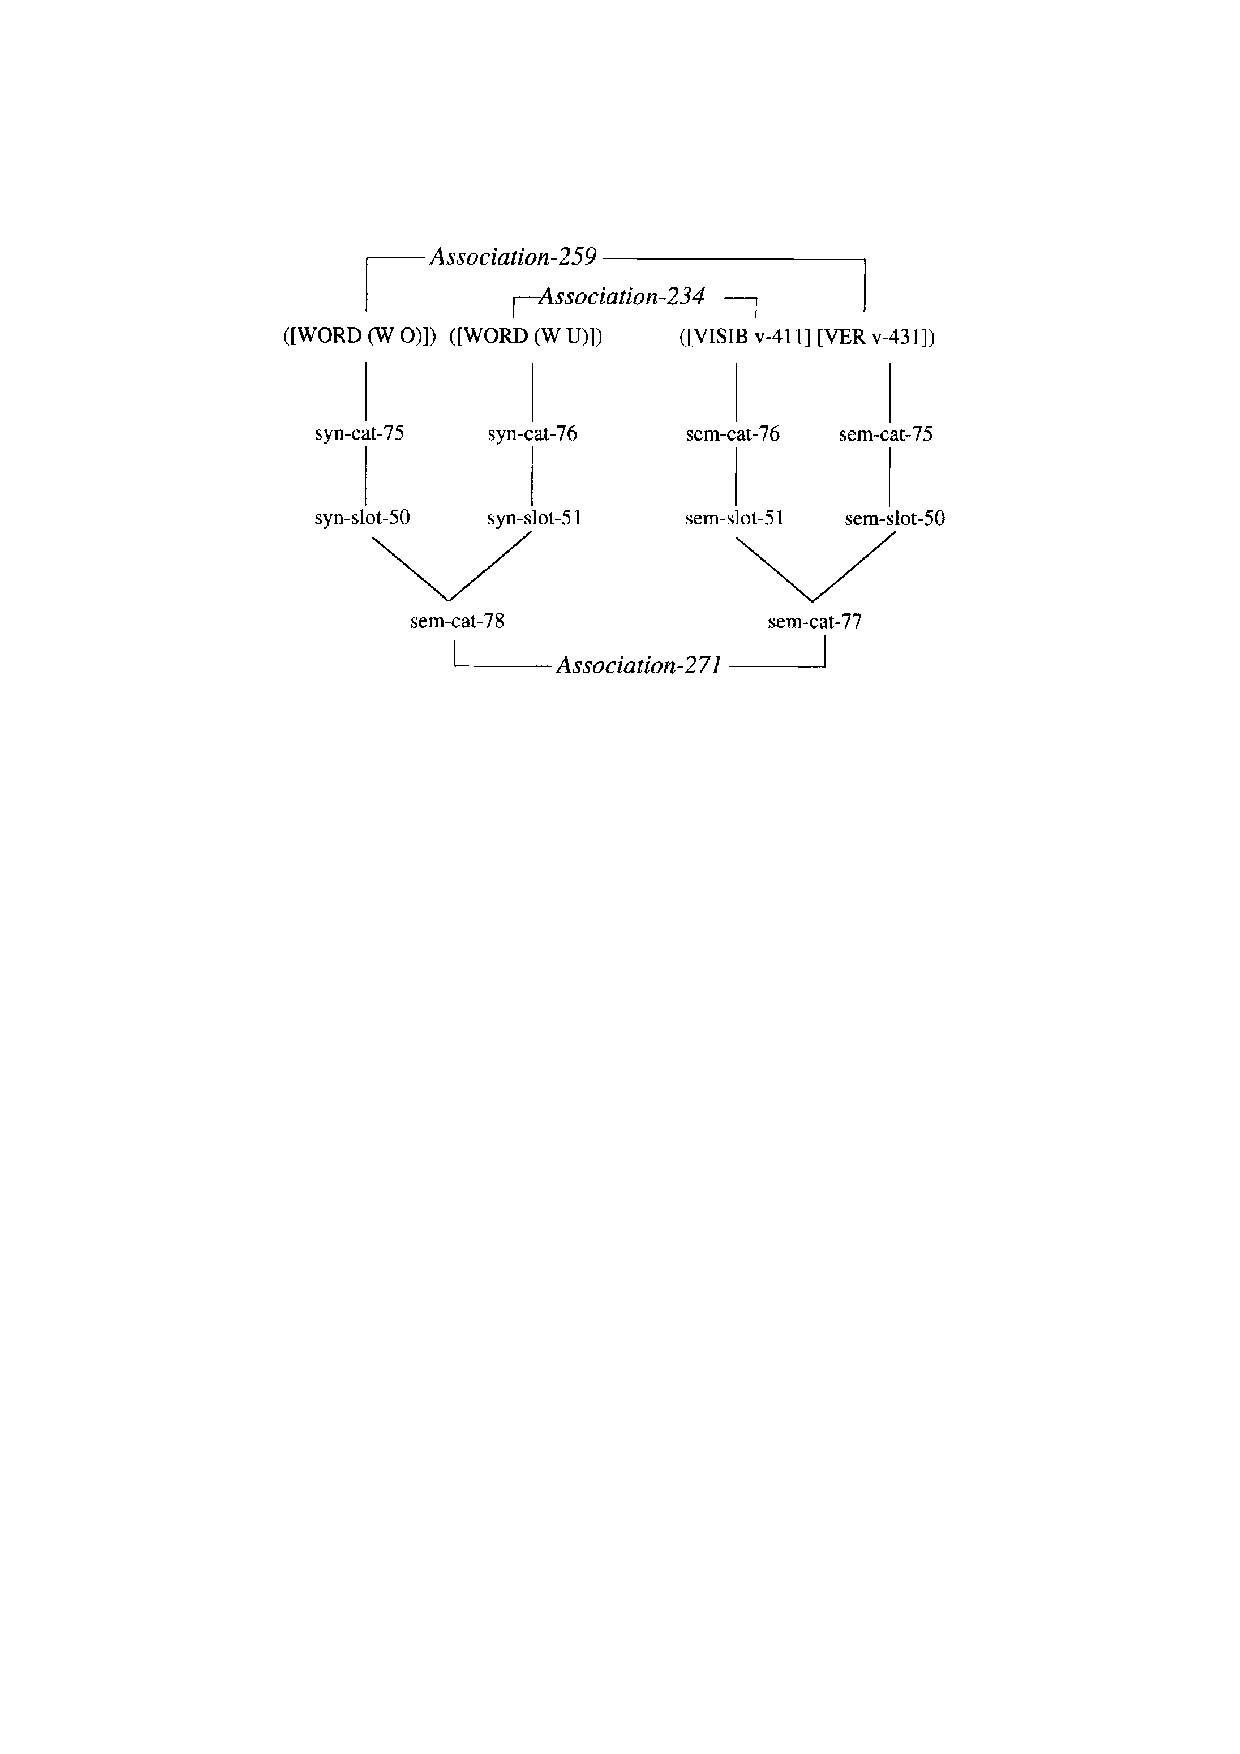
\includegraphics[width=0.75\textwidth]{chap10/figs/associations}}
\caption{\label{fig:associations} 
Top: Two lexical associations have become active (association-259 and association-234) to cover the distinctive 
feature-set ([VISIB v-411] [VER v-431]) resulting from discrimination and perception. Bottom: 
The group of words and the meanings match with schemas forming part of a grammatical association that combines the words. }
\end{figure}
An application of these schemas in producing the utterance ''(W O) (W U)'' is represented in \figref{fig:associations} and shown 
here: 
\begin{verbatim}
127 ++> Speaker: head-40 Topic: 2 Context: 6 5 4 3 1 0
Categorial Perception:
  ([VISIB v-4111] [VER v-431])([VER v-4311] [AREA v-4061])
Lexicon lookup: (Association-259 Association-234)
Syntactic structure:
  (syn-cat-77
    (syn-slot-50 (syn-cat-75 |(W O)|))
    (syn-slot-51 (syr-cat-76 |(W U)|)))
Semantic structure:
  (sem-cat-78
    (sem-slot-50 (sem-cat-75 (VER v-431)))
    (sem-slot-51 (sem-cat-76 (VISIB v-411))))
Meaning:
  ([VISIB v-4111] [VER v-4311)
Expression: ((W 0) (W U))
\end{verbatim}

So this experiment already contained several kernel ideas that would become the basis of further developments towards
computational formalisms that could handle evolutionary language game experiments, such as the 
representation of the grammar in terms of form-meaning pairs - similar to the lexicon - ,  
the use of schemas to represent the syntactic and semantic pole of a coupled feature structure, and the use of constraints to specify the 
properties of each pole, so that the grammar can be used in a bi-directional fashion. 
The relationship to construction grammar, which came to the foreground in linguistics 
around 1995, was not yet clear at the time. 

The paper also briefly described the mechanisms by which such a grammar emerged in the experiment in terms of a 
cognitive memory system: ''The cognitive memory system acts in a first instant purely as a device that records 
a particular way in which language has been produced so that it can later be re-produced in the same way.
Also the hearer can perform this recording operation. He is presented with a specific set of word forms from which he can abstract a syntactic schema. He derives meaning from the definition of the words in the lexicon and the distinctive feature-set coming out of perception. From this, a semantic schema can be extracted.
More interesting grammars emerge when additional operations to restructure the set of grammatical associations are used. For example, in the case of a partial match, substructures may be recategorized so that they nevertheless fit, two partially overlapping schemes with common fillers may lead to a new schema that integrates both, etc."

So the paper also contained already the kernel of ideas that would form the basis of grammatical experiments conducted many 
years later. However at that time the grammar formalism was still too weak to allow significant testing, let alone deal with more  
realistic features of grammar. Only after the Talking Heads experiment was finished, could more serious efforts towards 
grammar start in earnest.

\subsection{The Case Grammar Experiments}

The first of these efforts started around 2001 and focused on case grammar, i.e. on 
how grammatical constructions for expressing the arguments of a predicate describing a relation or
event could emerge and convergence in \is{Case Grammar experiment}
a population of grounded agents. Case grammar is one of the core functions of grammar and focusing on this domain would 
guarantee that we are addressing empirically attested core phenomena of human language. The first wave of work on case grammar
took place from 2001 to 2003. 
It required the construction of a more sophisticated vision system (accomplished by Jean-Christophe Baillie) and the 
design and implementation of a more sophisticated grammar formalism (accomplished by Luc Steels and Nicolas Neubauer), 
although this was still only one step on the way towards later developments in Fluid Construction Grammar. 

Based on these components, I implemented an initial experiment with only two agents.\footnote{
These experiments were first reported at the Harvard Evolution of Language conference in 2002 with a paper by Luc Steels
entitled `Computer Simulations of the origins of Case grammar'. The paper was later deemed 
``too incomprehensible for the Evolution of Language community'' to be acceptable for the conference 
proceedings edited by Maggie Tallerman.}
In 2005 Remi van Trijp picked up this line of research again and worked out the experiment 
further with great skill and sophistication. He extended the 
2-agent simulation to a multi-agent simulation and could finally report a complete running system in his 2008 Ph.d 
thesis.\cite{VanTrijp:2014}. Here I give only a brief account of the first attempts towards case grammar
and how this pushed the state of the art in language game research. 

But first we need a clearer idea on what case grammar is.
In the sentence ``John gave Mary a book", John plays the role of agent, the giver 
of the book, Mary that of recipient or 
beneficiary and the book is the `patient' or object of the action. Languages differ in terms of the strategies that they 
use to express these participant roles. Some of them, like German, have an elaborate system of morphological 
markers attached to constituents of the noun phrase. These markers signal that the 
phrase is nominative, accusative, dative, etc., and these cases then map in complex ways 
onto semantic roles such as agent and patient.
Other languages, like English, use a strategy based on word order and prepositions. For example, 
``Mary gave John a book'' contains the same participants as ``John gave Mary a book'' but now Mary is the 
agent and John the recipient. Still other languages, like Japanese, use a strategy based on particles following 
the noun, as in the Japanese sentence'' ''Tanaka-san wa Tokyo de o-to-san ni atta'' 
meaning Tanaka met his father in Tokyo. Tanaka-san is the name of a person, oto-san means ``father'' and atta 
means ``met". The markers are ``wa'' for the topic, ``de'' for location and ``ni'' for another sense of location which can 
also function as possessive. The case grammar experiments focused on modeling the latter strategy. 

It used the comparative method again to compare three progressively more complex strategies: 
\begin{enumerate}
\item {\bfshape  Lexical strategy}. The experiment starts from a purely 
lexical language that is predefined in all agents. The lexicon contained words for expressing properties of 
objects (such as ``smooth", ``red", etc.)
as well as actions involving objects (such as ``move-away-from", ``move-towards'' or ``push"). English words
were chosen to make the experiment easier to follow. Agents form
multi-word utterances using straightforward lexicon lookup, producing utterances
like ``move-towards red jill'' (Jill moves towards the red object) or ``push 
jack jill green'' (Jack pushes the green block to Jill). There is no syntax at all. Agents can nevertheless already 
achieve communicative success when they use the real world as a way to figure out the particant roles, even though the 
utterance does not provide any information. For example, to detect whether Jack pushes the green block to Jill or Jill 
pushes the green block to Jack. 

\item {\bfshape  Specific marker strategy}. The second strategy introduces markers in the form of particles added to words referring 
to objects, in order to specify what agument the object fills in the predicate describing the 
event. For example, there could be two markers: ``pi'' 
and ``pa'' specifying that the referent plays the role respectively of giver and gift in a give event, as in
"pi jill pa block give". The markers are entirely specific for each event in the sense that there is no generalisation 
yet to 'agent', 'patient' or other more abstract semantic roles. This already yields a more effective 
communication system because the complexity of seeking an interpretation matching with the world model is heavily
reduced and residual ambiguity (i.e. there is still more than one way in which the 
meaning matches with the world model) is also avoided. 

\item {\bfshape  Role strategy}. The third strategy introduces generalisations of the markers, so that 
fewer markers are needed. This decreases the size of the inventory and thus makes the language more efficient to 
process and easier to learn. There are many strategies that could be used for generalisation. Our experiments 
have explored the use of analogy: When arguments 
need to be expressed for an event e, agents no longer create new specific markers for each argument of e
but look for analogies between this event e and other events for which markers already exist. If a good analogy 
can be found they reuse it and generalise the argument-specific marker. 
\end{enumerate}
This analogy-based method of generalisation is explained in some more detail later in this section, but first 
we look briefly at other advances that were needed: What world was made available to the agents for their 
language games? How did the vision system work? And what grammatical formalism was devised to handle case grammar? 


\begin{figure}[htbp]
  \centerline{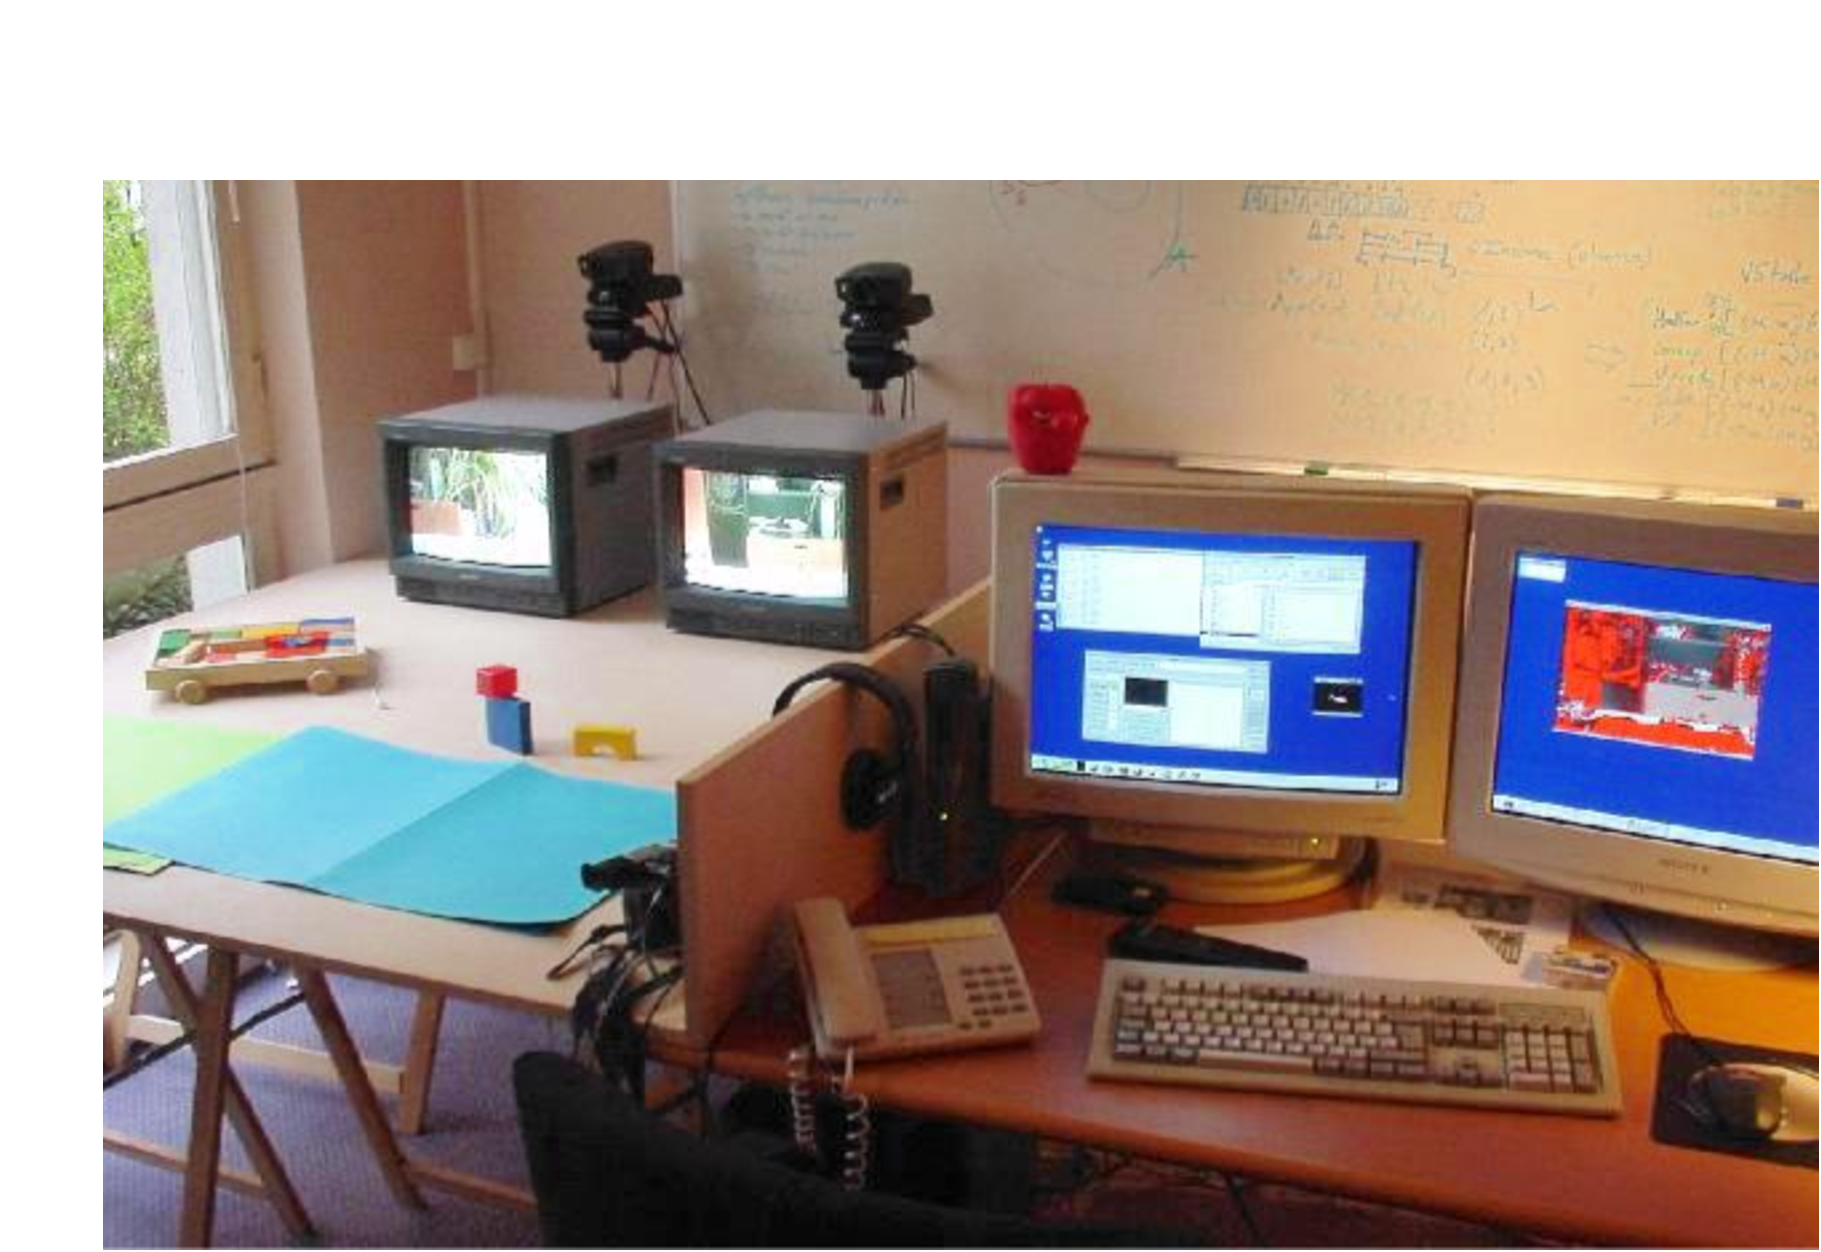
\includegraphics[width=.60\textwidth]{chap10/figs/peract-setup}}
\caption{\label{fig:peract-setup} 
The installation for the case grammar experiments used a more sophisticated vision system and objects that 
could be moved around. We see the two Talking Heads cameras in 
the background. They are oriented towards objects on the table or situations in the 
environment. The monitors show the camera images and the states of image processing, just as for the original 
Talking Heads experiment. 
}
\end{figure}

We used a similar set-up as the Talking Heads experiment (see \figref{fig:peract-setup}), but 
the world had to be made more complex, involving dynamical scenes in which 
different animate objects performed actions. So I decided to use 
puppets and enacted little scenes before the cameras (see \figref{fig:adam-eve} middle and bottom). 
There were two puppets, named Jack and Jill. They were actually sold at that time as puppet versions of Harry 
Potter and Hermelien Griffel inspired by the famous Harry Potter book series. 
The puppets appeared and disappeared within the field of view of the cameras. 
They manipulated small objects, for example pushing a green cube, picking it up, sliding the cube
towards the other puppet, putting it in a box, etc. To make the simulation more lively and easier to follow for 
a lay public, the agents engaging in a language game were also visually animated (see 
\figref{fig:adam-eve} top).\footnote{The animations were developed by Veronique Caraux in Paris.}


\begin{figure}[htbp]
  \centerline{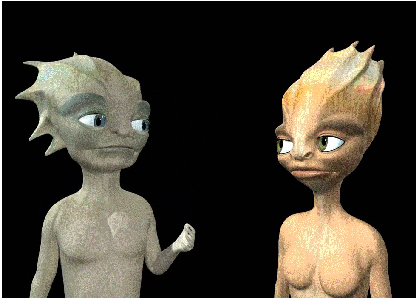
\includegraphics[width=.40\textwidth]{chap10/figs/adam-eve}}
\centerline{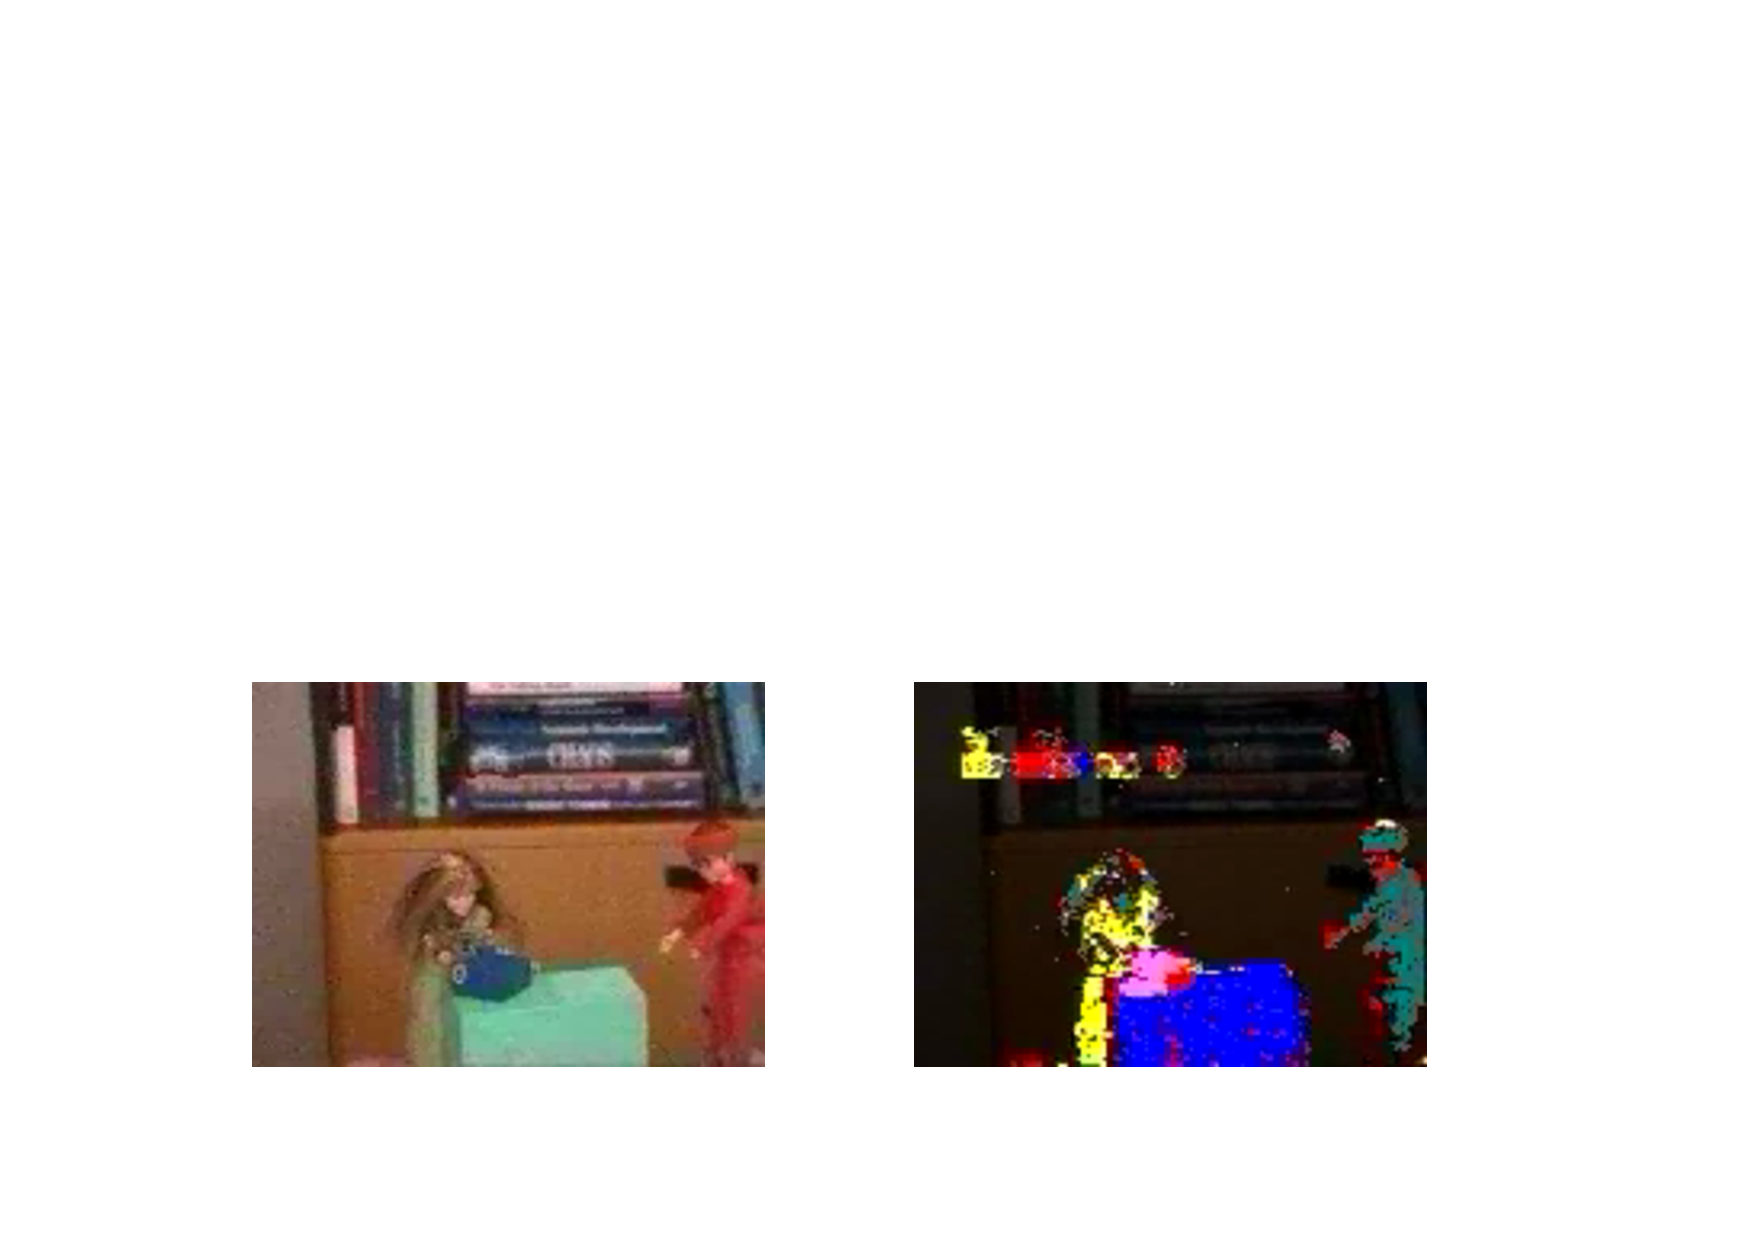
\includegraphics[width=.70\textwidth]{chap10/figs/jack-give}}
\centerline{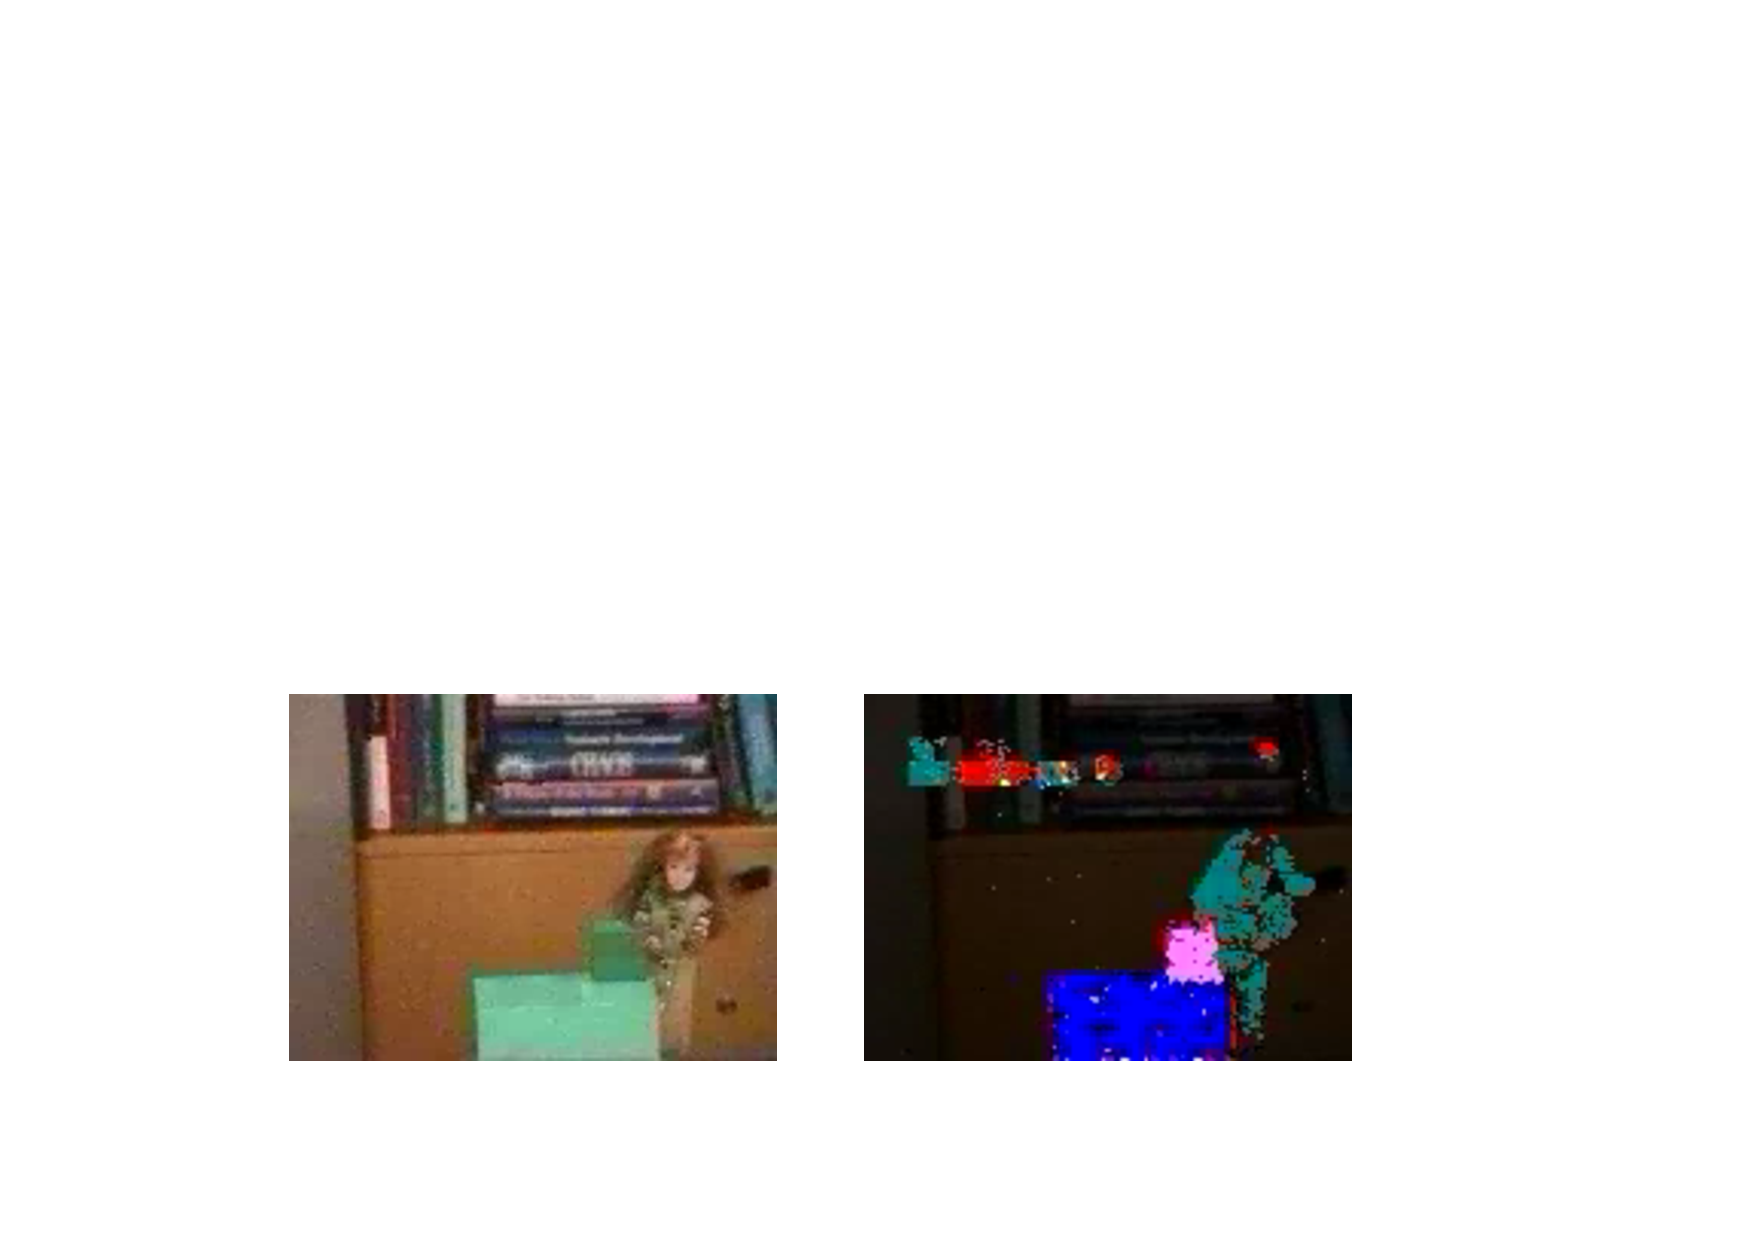
\includegraphics[width=.80\textwidth]{chap10/figs/push-jill}}
\caption{\label{fig:adam-eve} 
Top: Computer animation of the speaking and hearing agent used in public demonstrations 
of the case experiment. 
Middle: Example of a puppet scene, where Jill gives a block to Jack. It shows the source image (left) and a (partial) 
result of image processing (right). Bottom: Another example of a puppet scene where Jill pushes the block.}
\end{figure}

{\bfshape  Scaling up the vision system}\\

The vision system of the Talking Heads only dealt with static scenes. This had to be scaled up to
deal with dynamical scenes and event recognition. It was the focal work of 
Jean-Christophe Baillie at the Sony Computer Science Laboratory in Paris, who built a vision system 
called PERACT \is{PERACT vision system} inspired by an event-recognition developed by Jeffrey 
Siskind.\footnote{The vision system is described in the ph.D thesis of J-C Baillie. A summary is found here: 
\cite{Steels:2003}. Inspiration for the event recognition system came 
primarily from the paper by Siskind \cite{Siskind:2000}.}
The vision system was decomposed into three subsystems with information flowing both in a bottom-up
(from image to world model) and top-down way (from world model and predictions to image): the subsystems achieved 
object identification, event identification, and derivation of qualitative descriptors. 

{\bfshape  Object Identification} The first subsystem attempts to detect and track visual units at different hierarchical levels. 
It detects and 'latches onto' regions in the image that are generated by objects of 
interest in the environment. This results in deictic pointers or `anchors' that establish and monitor indexical references 
between internal symbols and external objects. Tracking not only takes place for a single object, but for 
an open-ended set of objects at different hierarchical levels, as long as they are part of the same spatio-temporal context. 

The detection and tracking of units at different hierarchical levels starts in a bottom-up manner from the images captured by the camera, and goes through various processing steps: figure/ground separation based on color perception, creation of a cellular occupancy grid, spatial region growing to identify spatial regions, and construction of spatio-temporal continuities based on 
color histograms of the objects (\figref{fig:peract-images}). 

\begin{figure}[htbp]
  \centerline{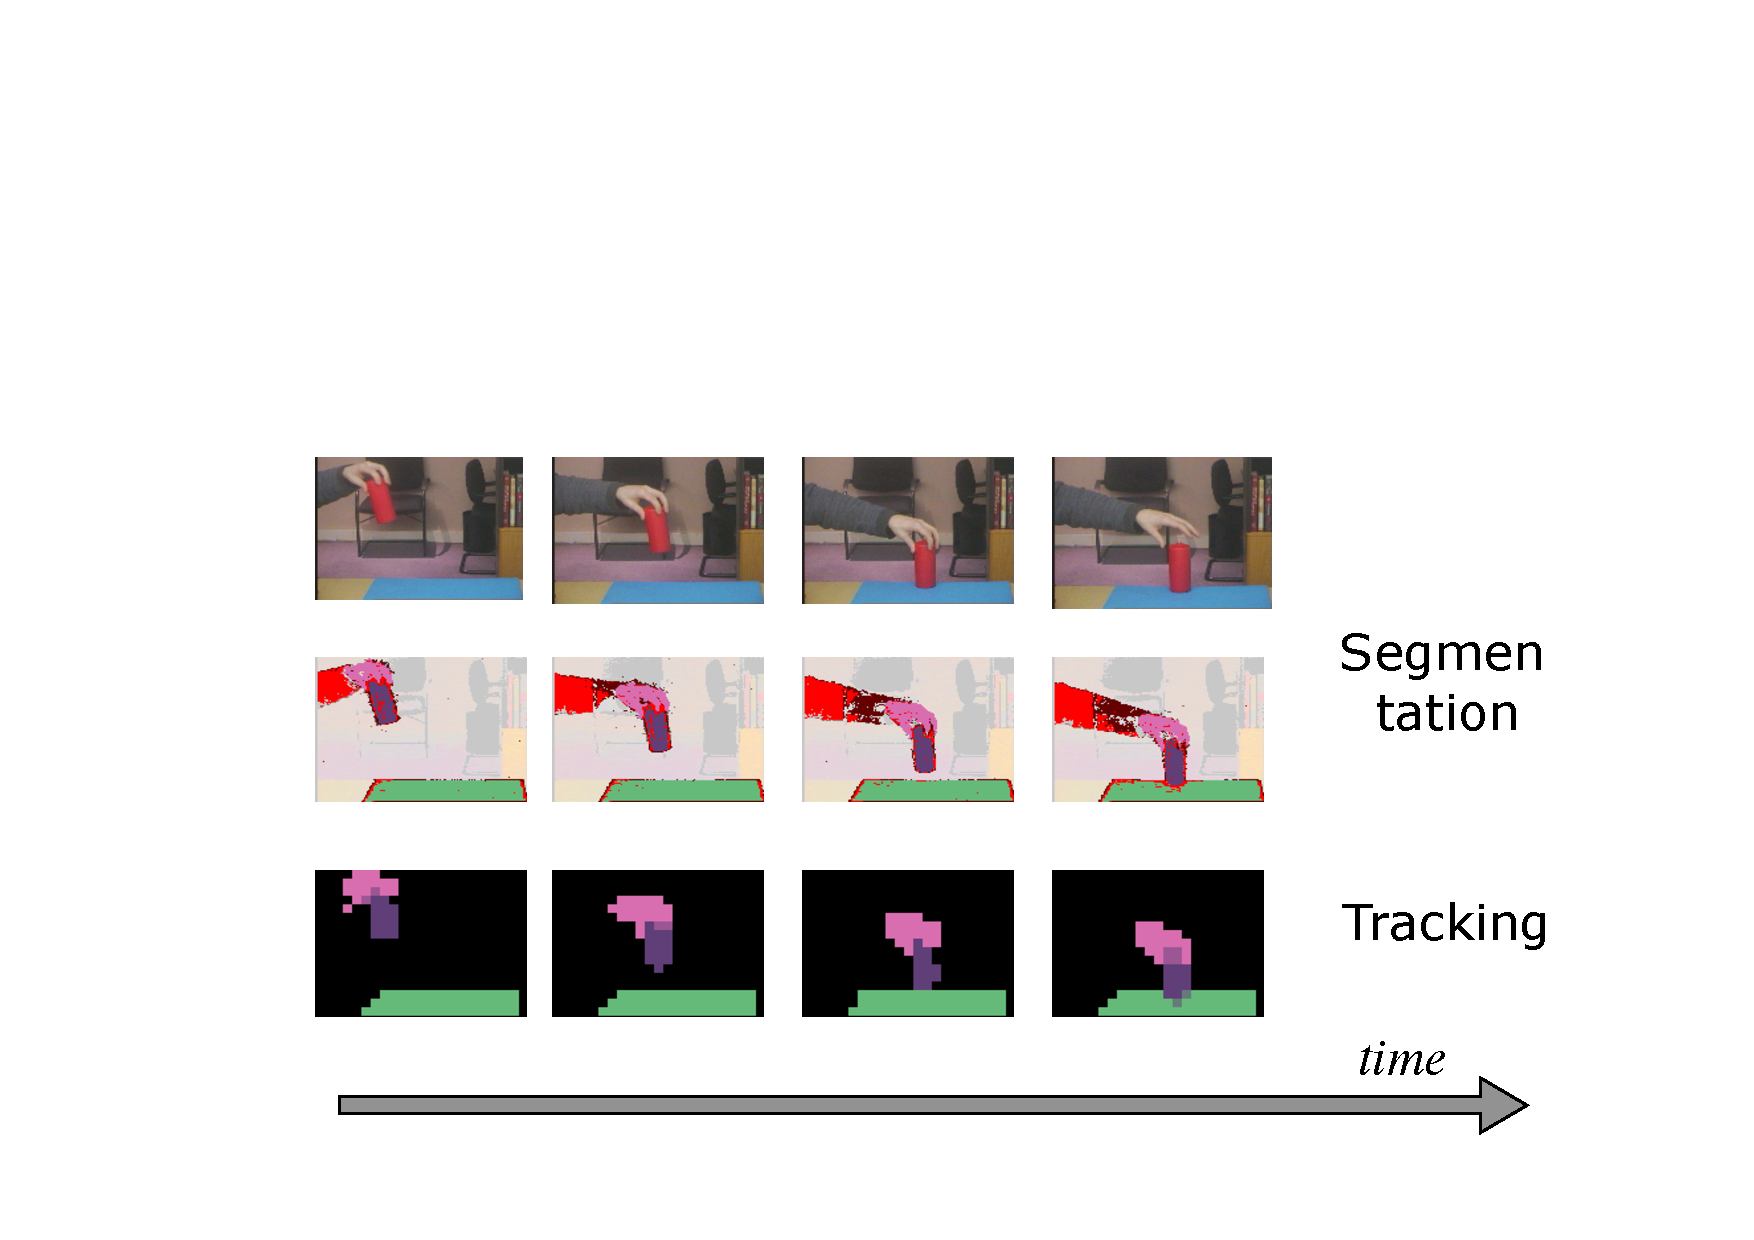
\includegraphics[width=.80\textwidth]{chap10/figs/peract-images}}
\caption{\label{fig:peract-images} 
Top: Some of the images recorded during the action of picking up a cylinder. 
Middle: Results of segmentation algorithms. 
Bottom: The spatio-temporal continuity of objects is tracked. 
}
\end{figure}

{\bfshape  Event Identification}

The second subsystem detects and tracks events, again at different hierarchical levels. The task is similar
to that of detecting objects but the grouping is based on changes in properties of objects rather than 
on invariances. Event detection is organised in three steps: 
\begin{enumerate}
\item Detect change by computing qualitative descriptions for the movement of an object, the contact between 
two objects, the approaching of two objects, the positioning of an object with respect to another one, etc. 
\item Detect micro-events by grouping image subsequences during which the same configuration 
of qualitative descriptors holds. 
\item Detect events which are defined as sequences of micro-events recognised using probabilistic state machines. 
For example a pick-up event (as in \figref{fig:peract-images}) involves three micro-events: (1) the hand 
moves towards the object, (2) the hand touches the object, and (3) both move away together. Processes 
concerned with recovering such events use a library of event definitions which is matched against the stream of micro-events.
\end{enumerate}
An example of output from this subsystem is shown below. Each event has an index (e.g. 77), a time period (e.g. 
from 780 to 803), other events or properties that have played a role in recognising this event, a 
label (e.g. {\verb Appear}), and information of the status (like ongoing or finished). 

\begin{verbatim}
...
(77 780 803 ((780 2) (783 20)) Appear 5 ONGOING)
(89 784 810 ((784 5) (790 20)) Halt 5 ONGOING)
(87 780 919 ((780 118) (899 20)) Appear 1 ONGOING)
(87 780 924 ((780 123) (904 20)) Appear 0 ONGOING)
(82 904 928 ((904 20) (925 3)) Halt 0 FINISHED)
(95 900 933 ((900 12) (913 20)) Approach_Resttogether 1 5 ONGOING)
(93 904 933 ((904 8) (913 20)) Put 1 0 5 ONGOING)
(92 780 937 ((780 123) (904 33)) Appear 0 FINISHED)
(74 924 937 ((924 3) (930 7)) Resttogether_Moveawayfrom 0 1 FINISHED)
(97 900 944 ((900 23) (924 20)) Halt 1 ONGOING)
(93 929 958 ((929 8) (938 20)) Halt 0 ONGOING)
(80 929 1017 ((929 8) (938 79)) Halt 0 FINISHED)
(91 938 1038 ((938 79) (1018 20)) Appear 0 ONGOING)
 ...
\end{verbatim}

{\bfshape  Qualitative Descriptors} 
The third subsystem consists of feature detectors that attempt to find qualitative descriptions for units at different levels 
of the object or event hierarchy. The result of all these processes is a set of streams, reporting objects and their 
properties dynamically in response to a changing world as well as the roles these different objects play in the events. 
A (short term) memory of these streams is kept as events unfold. It is used by the semantic system to construct or 
interpret the semantic structures that have to be expressed. Here is a small snapshot of the state of 
this visual memory with time stamps when the states occurred. 

\begin{verbatim}
... 
(CAUSE-MOVE-INSIDE ev-7 TRUE) <15:50:2>
(CAUSE-MOVE-INSIDE-TARGET ev-7 obj-1) <15:50:2>
(CAUSE-MOVE-INSIDE-PATIENT ev-7 obj-2) <15:50:2>
(CAUSE-MOVE-INSIDE-AGENT ev-7 YOU) <15:50:2>
(HALT ev-3 TRUE) <15:49:41>
(HALT-ARG ev-3 obj-1) <15:49:41>
(MOVE ev-1 TRUE) <15:49:24>
(MOVE-ARG ev-1 obj-1) <15:49:24>
(STRIPED obj-2) <15:48:42>
(HUGE obj-2) <15:48:42>
(BALL obj-2) <15:48:42>
(WHITE obj-2) <15:48:42>
(OBJECT obj-2) <15:48:42>
(STRIPED obj-1) <15:48:42>
(BIG obj-1) <15:48:42>
(PYRAMID obj-1) <15:48:42>
(YELLOW obj-1) <15:48:42>
(OBJECT obj-1) <15:48:42>
 ...
\end{verbatim}

Since this pioneering vision work, subsequent language game experiments on robots have all been using 
similarly sophisticated vision systems and currently such systems are standard components on commercially available
robots. 

{\bfshape  Scaling up the language system}\\

Not only the vision system, but also the language system had to be scaled up significantly to do these experiments. 
Together with Nicolas Neubauer, I built upon the formalism I had developed for the early syntax experiments, 
designing and implementing a next generation system, called COGAR, \is{COGAR (cognitive grammar architecture)} which stands for 
Cognitive Grammar Architecture.\footnote{
No official publication of the COGAR system exists. Such technical papers are virtually impossible to get 
published in journals or conferences. There was however a technical report \cite{Steels:2001}.}
Here is a brief description of this formalism. 

COGAR represents syntactic and semantic structures as frames with units, slots and 
constraints on the slots. The frames are in many ways similar to the feature structures used in feature-structure 
based grammars such as HPSG, although there are many important differences. For example, each unit has a 
unique name so that it becomes possible to refer back to units in defining constraints. COGAR also used 
logic variables (denoted by a symbol with a question mark in front) as opposed to path descriptions, which 
lead to the adoption of techniques from logic programming 
The syntactic and semantic structure of a particular utterance are coupled together as a coupled feature structure 
by making the unit-names shared. Often both are combined when the coupled feature structure needs to be displayed
as in this example below. 
\begin{verbatim}
((unit-15
   (scope utterance)
   (subunits (unit-17 unit-18 unit-16))
   (ordering (unit-17 unit-18 unit-16)))
 (unit-17
   (form (smooth))
   (meaning ((smooth ?source-object1)))
   (referent ?source-object1) 
   (gramcat (takes-marker-1)))
 (unit-18 (form (po)))
 (unit-16 
   (form (move-away-from)) 
   (meaning
     ((move-away-from ?event ?state) 
      (move-away-from-1 ?event ?object)
      (move-away-from-2 ?event ?source-object1)))))
\end{verbatim}
This example could have been constructed, either in parsing or producing, for 
the utterance ``po smooth move-away-from". Syntactic properties such as the form of the word, 
the ordering of the units, or the grammatical categories of a unit are represented explicitly on the syntactic side and 
the meaning and referent are represented on the semantic side. In general, COGAR allows the representation of
any kind of information at whatever level of linguistic analysis as part of a feature structure. 

Notice that the arguments for a predicate describing an event are decomposed into separate predicates, one for 
each argument. For example move-away-from (?event,?object,?source-object) has three arguments and this 
is decomposed into three expressions: 
\begin{verbatim}
  (move-away-from ?event ?state) 
  (move-away-from-1 ?event ?object)
  (move-away-from-2 ?event ?source-object)
\end{verbatim}
?state is bound to true, false or unknown. 

The lexicon and grammar in COGAR takes the form of a set of bi-directional rules. The rules have two poles 
which are typically the semantic and syntactic pole, although there could be rules that work only on the 
syntactic level and others that work on the semantic level. The rules are applied 
from right to left in production and from left to right in parsing. 
The rules can have variables at any position and in anyone of the two poles. In order to be applicable, 
one pole of the rule has to match, which means that the structure defined in the pole had to 
have correspondents within the target structure, possibly after binding the variables to concrete 
symbols in the coupled feature structure. If a complete match is 
found, the other pole is merged with the target, which means that all variables get instantiated and every 
element which is not yet in the target is added. The underlying computational model of COGAR  
is therefore similar to a rule-based inference system, with an inference engine that cycles through the rules until 
no more rules can be applied. The variables are logic variables and hence the matching and merging is similar 
to the process of unification as used in PROLOG or other logic programming languages. 

Here is an example of a lexical rule that defines the meaning of the word for an event ``move-away-from". The referent is 
the object that is referred to by the word, in this case it is the event itself. 
\begin{verbatim}
((?unit 
   (meaning
      (== (move-away-from ?event ?state)
          (move-away-from-1 ?event ?object)
          (move-away-from-2 ?event ?source)))
   (referent ?event)) 
<-->
((?unit
   (form (== move-away-from)))))
\end{verbatim}
Next, here is an example of a rule for the marker ``po". On the semantic side it ensures that the referent of one unit 
whose referent is ?source is equal to the object filling the argument move-away-from-2 in a move-away-from event. 
On the syntactic side, it triggers when there is a word that has the grammatical category `takes-marker-1' and 
is preceded by the marker ``po". (<< stands for 'preceeds') 
\begin{verbatim}
((?predicate 
   (meaning
    (== (move-away-from ?evnt)
        (move-away-from-1 ?evnt ?patient)
        (move-away-from-2 ?evnt ?source))))
 (?argument
   (referent ?source))) 
<---> 
((?argument
   (gramcat (== takes-marker-1)))
 (?marker-unit
   (form (== po))) 
(<< ?marker-unit ?argument))))
\end{verbatim}

There are additional rules that specify which word takes which marker, by assigning them to a particular 
grammatical category. For example, the word ``smooth'' has the category `takes-marker-1': 
\begin{verbatim}
((?unit
   (gramcat (== takes-marker-1)) 
   (form (== smooth))))
<---> 
((?unit (form (== smooth))))
\end{verbatim}

The marker ''po'' in the above example is entirely specific for one argument of the move-away-from predicate, as would be the 
case when the second strategy is enacted. To implement the third strategy 
(to achieve more abstract semantic roles) requires that the markers become generic, which implies that 
we get additional rules that recategorise the arguments of a predicate in terms of 
semantic roles like: agent, patient, source, etc. Here is an example of a rule that 
has this effect. role-1 is an example of a semantic role created by the agent as an abstraction of the 
move-away-from-2 argument. 
\begin{verbatim}
((?predicate
   (meaning
    (== (move-away-from ?evnt) (move-away-from-1 ?evnt ?patient)
        (move-away-from-2 ?evnt ?source)))))
<---> 
 ((?predicate
    (meaning
      (== (move-away-from ?evnt) (move-away-from-1 ?evnt ?patient)
          (move-away-from-2 ?evnt ?source)))) 
    (expanded-meaning (== (role-1 ?evnt ?source))))
\end{verbatim}
And the rules that click eveything together now operate over semantic roles as shown in the following example: 
\begin{verbatim}
 ((?predicate
   (expanded-meaning (== (role-1 ?event ?source))))
  (?unit (referent ?source))) 
<---> 
 ((?unit (gramcat (== takes-marker-1)))
  (?marker-unit (form (== po))) 
 (<< ?marker-unit ?unit))
\end{verbatim}
Recall that all rules must be reversible and that the conditional part must match and the concluding part must unify.\\

{\bfshape  Analogy as the driver of generalisation}\\

There is of course a lot more to say about how all this works computationally and about how these rules are built during 
learning. The reader is referred to references given earlier. 
But let us here just focus only on the very non-trivial question where role-abstractions 
like agent, patient, or source come from. Analogy, which is clearly a basic feature of human 
cognition in general, is proposed as the key mechanism. \is{analogy of semantic roles} When agents have to 
express which argument an object fills in an event, they first try to see whether there is already a marker that 
expresses an argument in an analogous event. When this is the case, the marker is first generalised to 
express a new semantic role (if it was not yet a role) and then the unexpressed event-argument is 
categorised in terms of this role. If the hearer encounters a new use of a marker, he will also use analogy to 
find the connection between the event used earlier on and the newly encountered event.

Operationalising analogy is extremely difficult because humans tend to incorporate almost anything in how they 
make analogical inferences and inferences are heuristic as opposed to rigid logical derivations. The analogical 
mapping used in the case grammar experiment starts from two events, further called the source-event, for which some relations have already been expressed, and the target event for which a marker needs to be constructed. The first step in analogy-making consists in decomposing both events into the primitive micro-events that the vision system is using to recognise the 
event. The second step is to find a mapping between them. 

Here is an example showing how the argument walk-to-1 is mapped onto the argument move-inside-1.
The walk-to event features two arguments, walk-to-1 (the agent walking) and walk-to-2 (the 
target towards which the agent is walking). It consists of four micro-events: The agent does not 
move, the target does not move, then the agent approaches the target, and then the agent touches the target. 
This means that the event 
\begin{verbatim}
  (WALK-TO-2 ev-100 JILL) (WALK-TO-1 ev-100 JACK) 
  (WALK-TO ev-100 TRUE)
\end{verbatim}
expands into:
\begin{verbatim}
  (MOVE ev-165641 TRUE) (MOVE-1 ev-165641 JACK)
  (MOVE ev-165419 FALSE) (MOVE-1 ev-165419 JILL)
  (APPROACH ev-165486 TRUE) (APPROACH-2 ev-165486 JILL)
  (APPROACH-1 ev-165486 JACK)
  (TOUCH ev-165633 TRUE) (TOUCH-2 ev-165633 JACK)
  (TOUCH-1 ev-165633 JILL)
\end{verbatim}
The move-inside event has also two arguments: move-inside-1 (the agent moving) and 
move-inside-2 (the location in which the agent is moving). It consists of eight 
micro-events: The agent is visible, the location is visible, the distance between the agent and 
the location decreases, the location does not move, the agent does not touch the location, 
then the agent touches the location, and then the agent becomes invisible. The 
following description of a move-inside event
\begin{verbatim}
 (MOVE-INSIDE ev-163190 TRUE) (MOVE-INSIDE-2 ev-163190 HOUSE-1)
 (MOVE-INSIDE-1 ev-163190 JILL)
\end{verbatim}
therefore expands into the following micro-events:
\begin{verbatim}
 (VISIBLE ev-161997 TRUE) (VISIBLE-1 ev-161997 JILL)
 (DISTANCE-DECREASING ev-162441 TRUE) 
    (DISTANCE-DECREASING-2 ev-162441 HOUSE-1) 
 (DISTANCE-DECREASING-1 ev-162441 JILL)
 (MOVE ev-161794 FALSE) (MOVE-1 ev-161794 HOUSE-1)
 (TOUCH ev-161801 FALSE) (TOUCH-2 ev-161801 HOUSE-1) 
    (TOUCH-1 ev-161801 JILL) 
 (TOUCH ev-162493 TRUE) (TOUCH-2 ev-162493 HOUSE-1) 
    (TOUCH-1 ev-162493 JILL)
 (VISIBLE ev-161791 TRUE) (VISIBLE-1 ev-161791 HOUSE-1) 
 (VISIBLE ev-162665 FALSE) (VISIBLE-1 ev-162665 JILL)
\end{verbatim}
Next each micro-event in the target-event is paired with all micro-events in the source-event which use the same predicate. Micro-events which cannot be mapped this way are ignored. The temporal information which is part of the hierarchical event description is not used either. For the mapping from the move-inside event to the walk-to event, we get the following result:
\begin{verbatim}
  move-inside event => walk-to event
 (TOUCH ev-162689 TRUE) => (TOUCH ev-165633 TRUE)
 (TOUCH-1 ev-162689 JACK) => (TOUCH-1 ev-165633 JILL)
 (TOUCH-2 ev-162689 HOUSE-1) => (TOUCH-2 ev-165633 JACK)
 (TOUCH ev-161796 FALSE) => (TOUCH ev-165633 TRUE)
 (TOUCH-1 ev-161796 JACK) => (TOUCH-1 ev-165633 JILL)
 (TOUCH-2 ev-161796 HOUSE-1) => (TOUCH-2 ev-165633 JACK)
 (MOVE ev-161794 FALSE) => (MOVE ev-165419 FALSE)
 (MOVE ev-165641 TRUE) (MOVE-1 ev-161794 HOUSE-1) => 
        (MOVE-1 ev-165419 JILL) (MOVE-1 ev-165641 JACK)
\end{verbatim}
A good mapping is such that the filler of the argument of interest (in this case 
Jack, which fills the move-inside-1 argument in the move-inside event) always maps onto the same object in 
the source-event. This is indeed the case here because Jill, which fills the role of move-inside-1 
in the walk-to event, always plays the same role in all source micro-events as Jack in the matching target micro-events. 
Note that walk-to-2 would not extend by analogy to move-inside-2 because the object house-1 (which fills the role 
of move-inside-2) maps onto different object roles in the source-event. 
Once the analogy established, the marker already available for the walk-to-1 event-object relation is 
re-used for marking the move-inside-1 relation. 

Here are some results from comparative experiments using real world data. 
The graph in \figref{fig:comparison} compares the number of markers that have been derived by the agents for two experiments, 
each using data from the same series of 1300 language games. The first experiment (top graph) does not 
use analogy, hence new markers are created for every argument in every predicate
that needs to be expressed. The grammars basically stabilise after about 700 games with 28 markers. In the second 
experiment (the two bottom graphs) the strategy with analogy has been used. There is a graph showing the 
growth in the number of role markers and another one in the number of argument markers. Agents 
generated 4 role markers in the second experiment, covering a wide range of events, and 7 more 
specific argument markers, which might still be generalised later. The grammars of the agents stabilised
much earlier after 200 games, which proves the point that the use of analogy not only results in 
a more compact grammar with more expressive power, but also in a grammar that is faster to emerge and 
easier to learn.  

\begin{figure}[htbp]
  \centerline{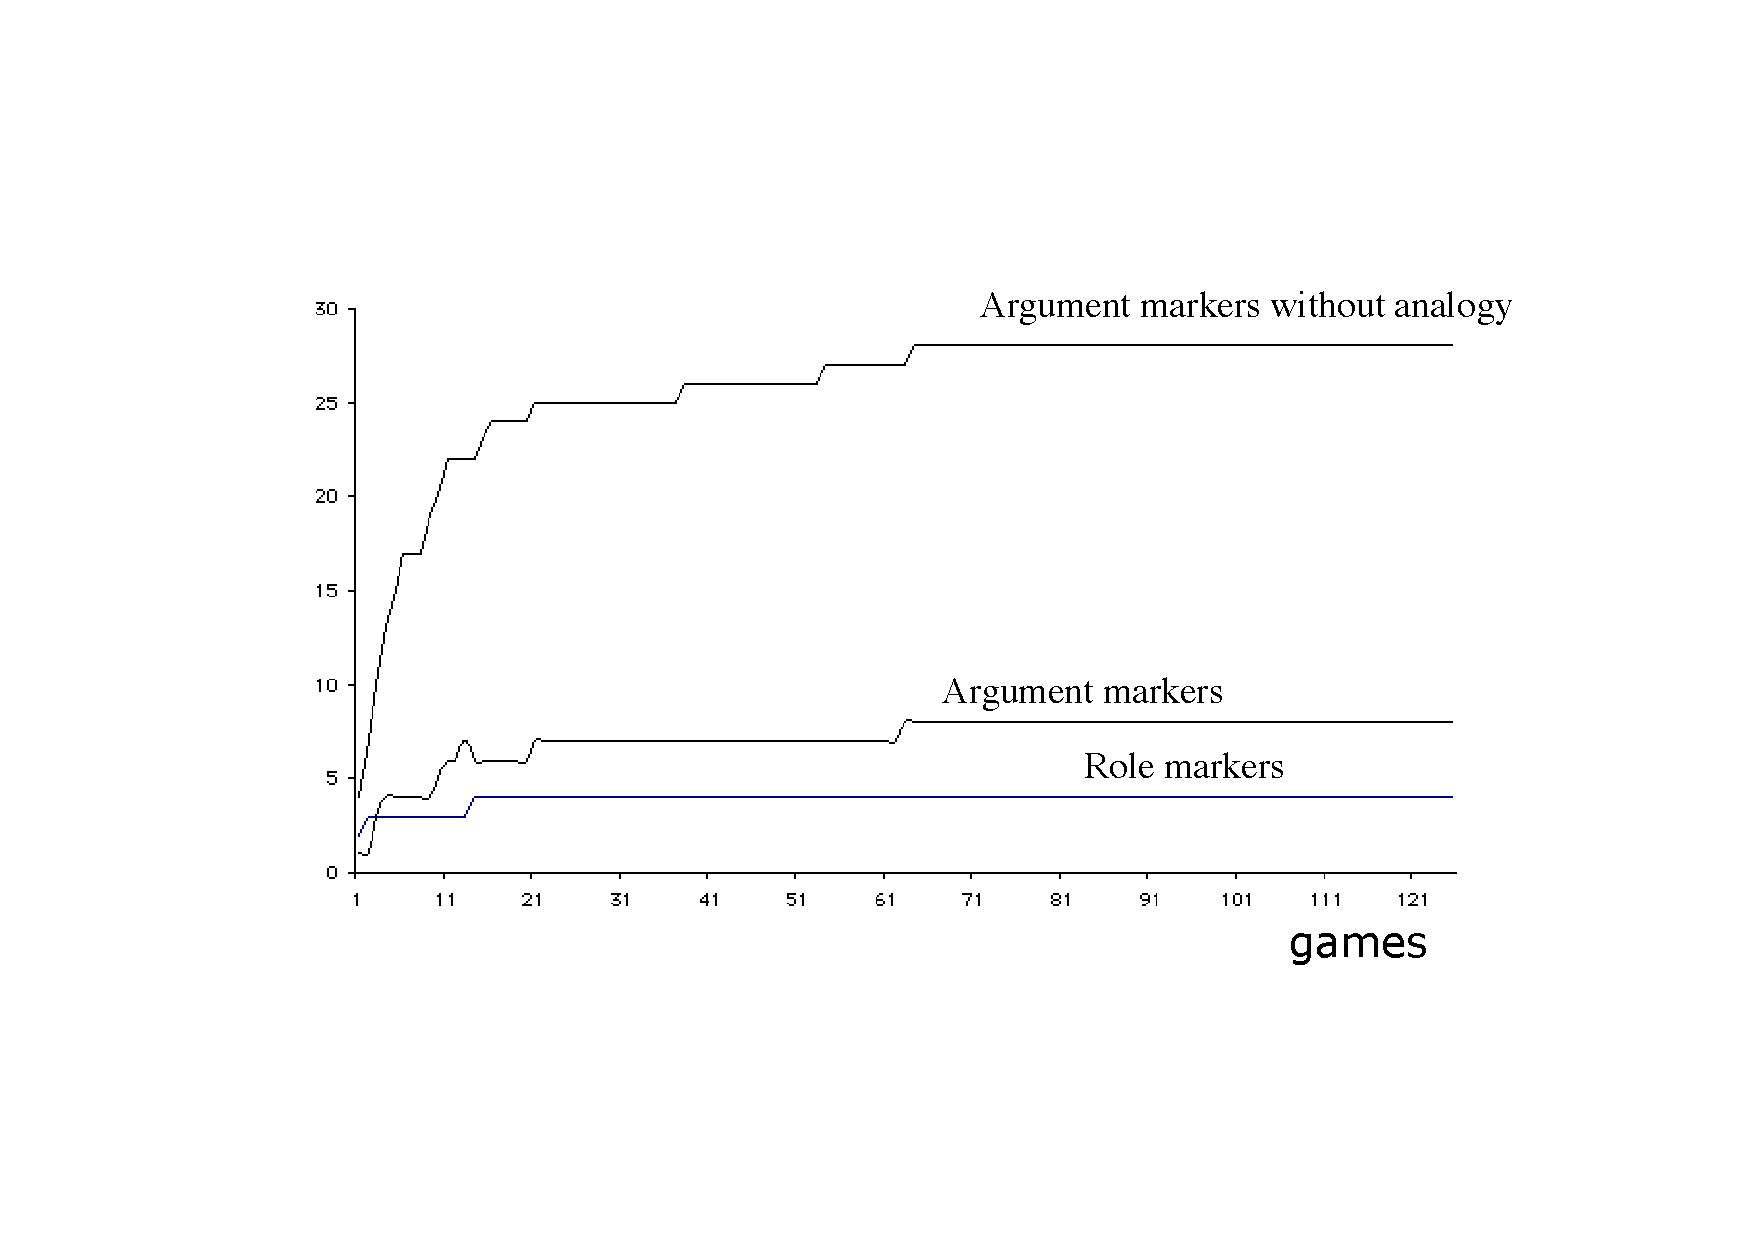
\includegraphics[width=.70\textwidth]{chap10/figs/comparison}}
\caption{\label{fig:comparison} 
Comparison between two different strategies: The top-graph shows the growth in the average number of 
markers for the event-specific marker strategy. 
The bottom two graphs show the average size of the set of markers when analogy is used. Overall, 
fewer markers are needed, making the case marking system more efficient and thus explaining why we 
get abstract semantic roles.}
\end{figure}

This first case experiment was only the beginning of more thorough and systematic research by Remi van Trijp who 
scaled up the experiment to multi-agent simulations and made several additional discoveries, such as the necessity 
to use multi-level alignment.\cite{Steels:07d} \is{multi-level alignment}
But the early experiment was already of huge importance to open the path towards realistic grammars. 
In parallel, other areas of grammars began to be tackled, 
particularly grammars for tense and aspect.\footnote{
Work on tense and aspect was first carried out by Joachim de Beule \cite{DeBeule:2004}, \cite{DeBeule:2006}
and then continued by Michael Spranger and Katya Gerasymova \cite{Gerasymova:2012}, 
although this domain still remains in an exploratory phase today.}

\section{Conclusions} 

This chapter described a first batch of language game experiments, happening at the same time or right after the Talking Heads 
experiment. They were beginning to climb slowly up on the long and winding path towards languages that are similar in 
complexity from the viewpoint of interaction, perception, conceptualisation and grammar to human natural languages. 
The research landscape was becoming clearer but at the same time the enormity of the challenges that remained
became obvious. There is clearly not a single simple mechanism that can explain all of language. Instead we have 
to do concrete case studies to advance the state of the art step by step, both for the explanation of concrete language 
phenomena such as perspective reversal or case grammar, and for finding the general theory that underlies the 
emergence and evolution of language. 

